% !TeX root = RJwrapper.tex
\title{brolgar: An R package to BRowse Over Longitudinal Data Graphically and Analytically in R}
\author{by Nicholas Tierney, Dianne Cook, and Tania Prvan}

\maketitle

\abstract{%
Longitudinal (panel) data provide the opportunity to examine temporal patterns of individuals, because measurements are collected on the same person at different, and often irregular, time points. The data is typically visualised using a ``spaghetti plot'', where a line plot is drawn for each individual. When overlaid in one plot, it can have the appearance of a bowl of spaghetti. With even a small number of subjects, these plots are too overloaded to be read easily. The interesting aspects of individual differences are lost in the noise. Longitudinal data is often modelled with a hierarchical linear model to capture the overall trends, and variation among individuals, while accounting for various levels of dependence. However, these models can be difficult to fit, and can miss unusual individual patterns. Better visual tools can help to diagnose longitudinal models, and better capture the individual experiences. This paper introduces the R package, \CRANpkg{brolgar} (BRowse over Longitudinal data Graphically and Analytically in R), which provides tools to identify and summarise interesting individual patterns in longitudinal data.
}

\hypertarget{introduction}{%
\section{Introduction}\label{introduction}}

This paper is about exploring longitudinal data effectively. By ``longitudinal data'' we specifically mean individuals repeatedly measured through time. This could include panel data, where possibly different samples from a key variable (e.g.~country), are aggregated at each time collection. The important component is a key variable with repeated measurements regularly, or irregularly over time. The inherent structure allows us to examine temporal patterns of individuals, shown in Figure \ref{fig:heights-sample-plot}, of the average height of Australian males over years. The individual component is \texttt{country}, and the time component is \texttt{year}. The variable \texttt{country} along with other variables is measured repeatedly from 1900 to 1970, with irregular intervals between years.

\begin{figure}

{\centering 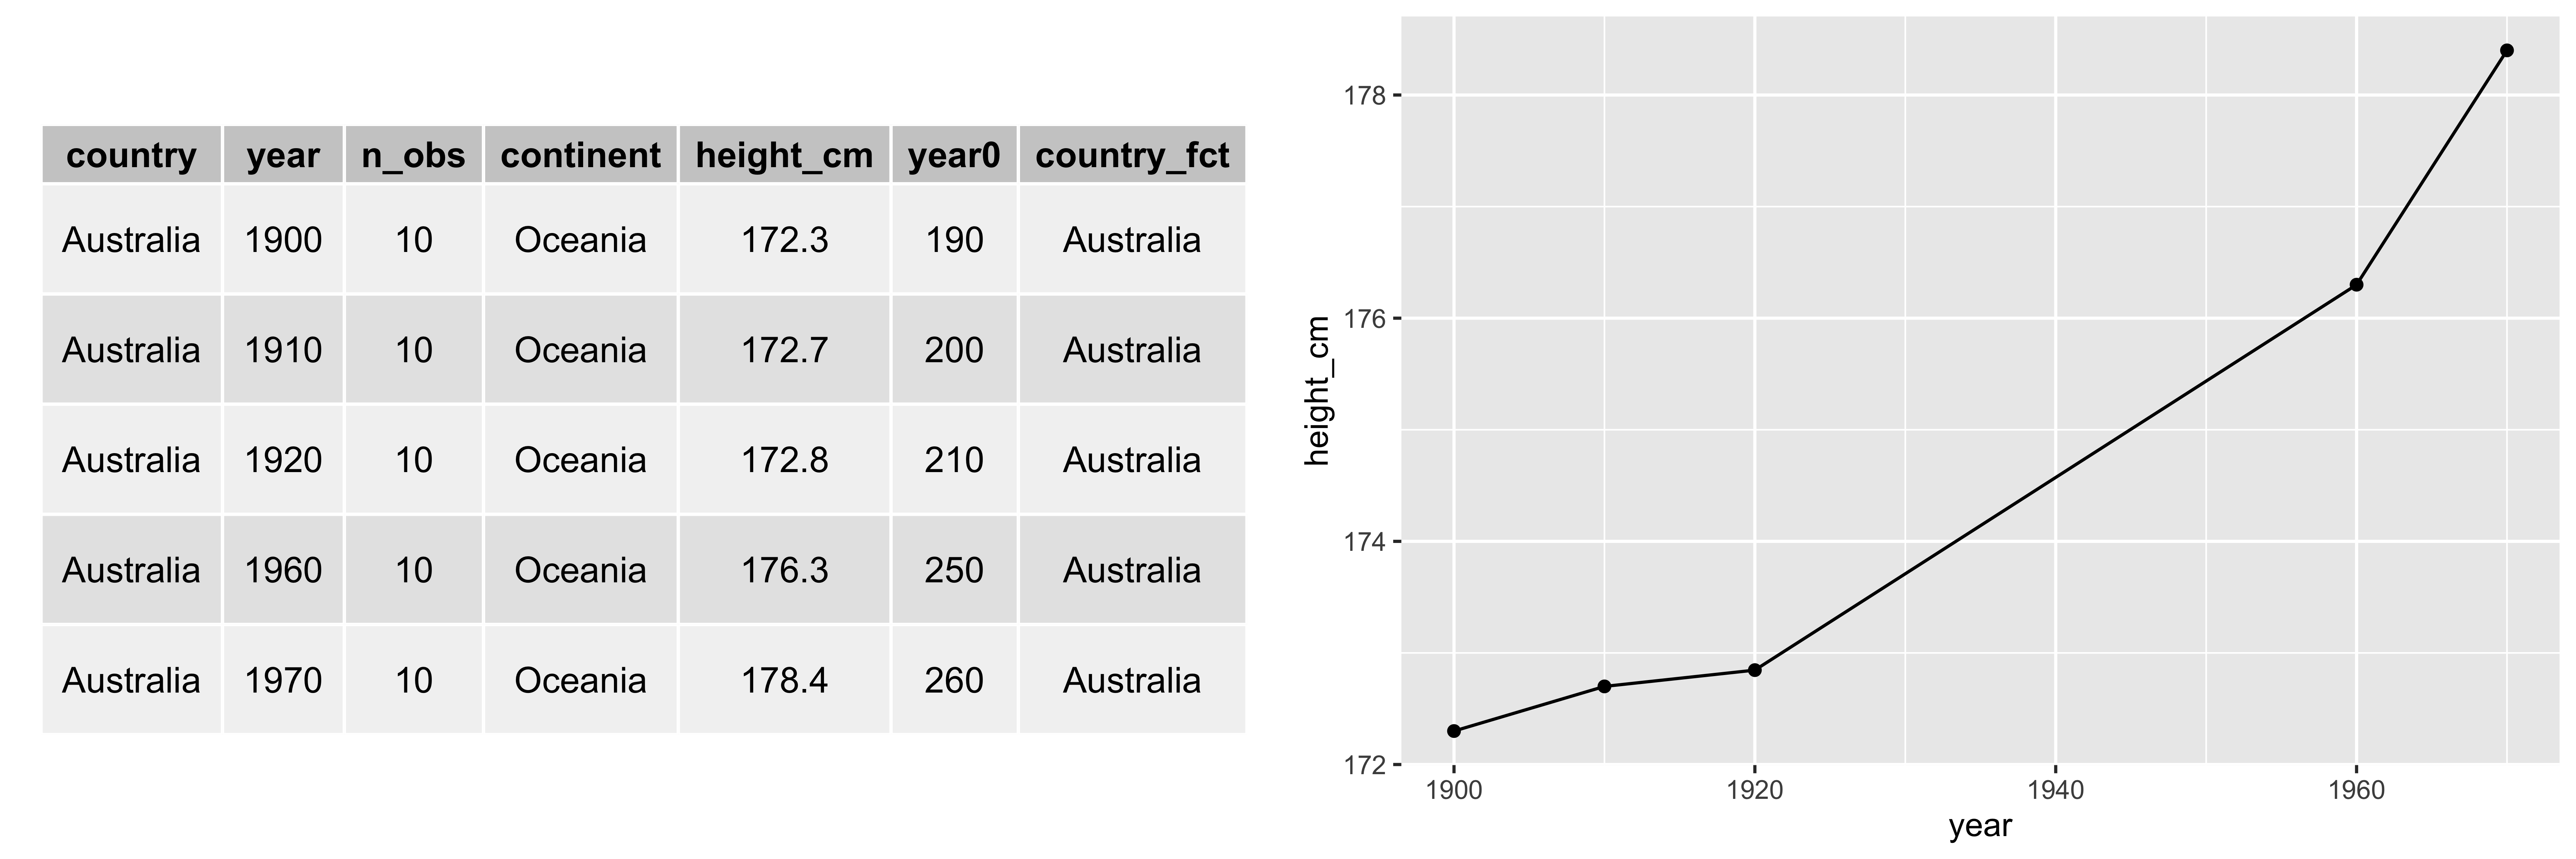
\includegraphics[width=0.95\linewidth]{brolgar-paper_files/figure-latex/heights-sample-plot-1} 

}

\caption{Example of longitudinal data: average height of men in Australia for 1900-1970. The height increase over time, and are measured at irregular intervals.}\label{fig:heights-sample-plot}
\end{figure}

The full dataset of Figure \ref{fig:heights-sample-plot} is shown in Figure \ref{fig:spaghetti}, showing 144 countries from the year 1700. This plot is challenging to understand because there is overplotting, making it hard to see the individuals. Solutions to this are not always obvious. Showing separate individual plots of each country does not help, as 144 plots is too many to comprehend. Making the lines transparent or fitting a simple model to all the data Figure \ref{fig:spaghetti}B, might be a common first step to see common trends. However, all this seems to clarify is: 1) There is a set of some countries that are similar, and they are distributed around the center of the countries, and 2) there is a general upward trend in heights over time. We learn about the collective, but lose sight of the individuals.

\begin{figure}

{\centering 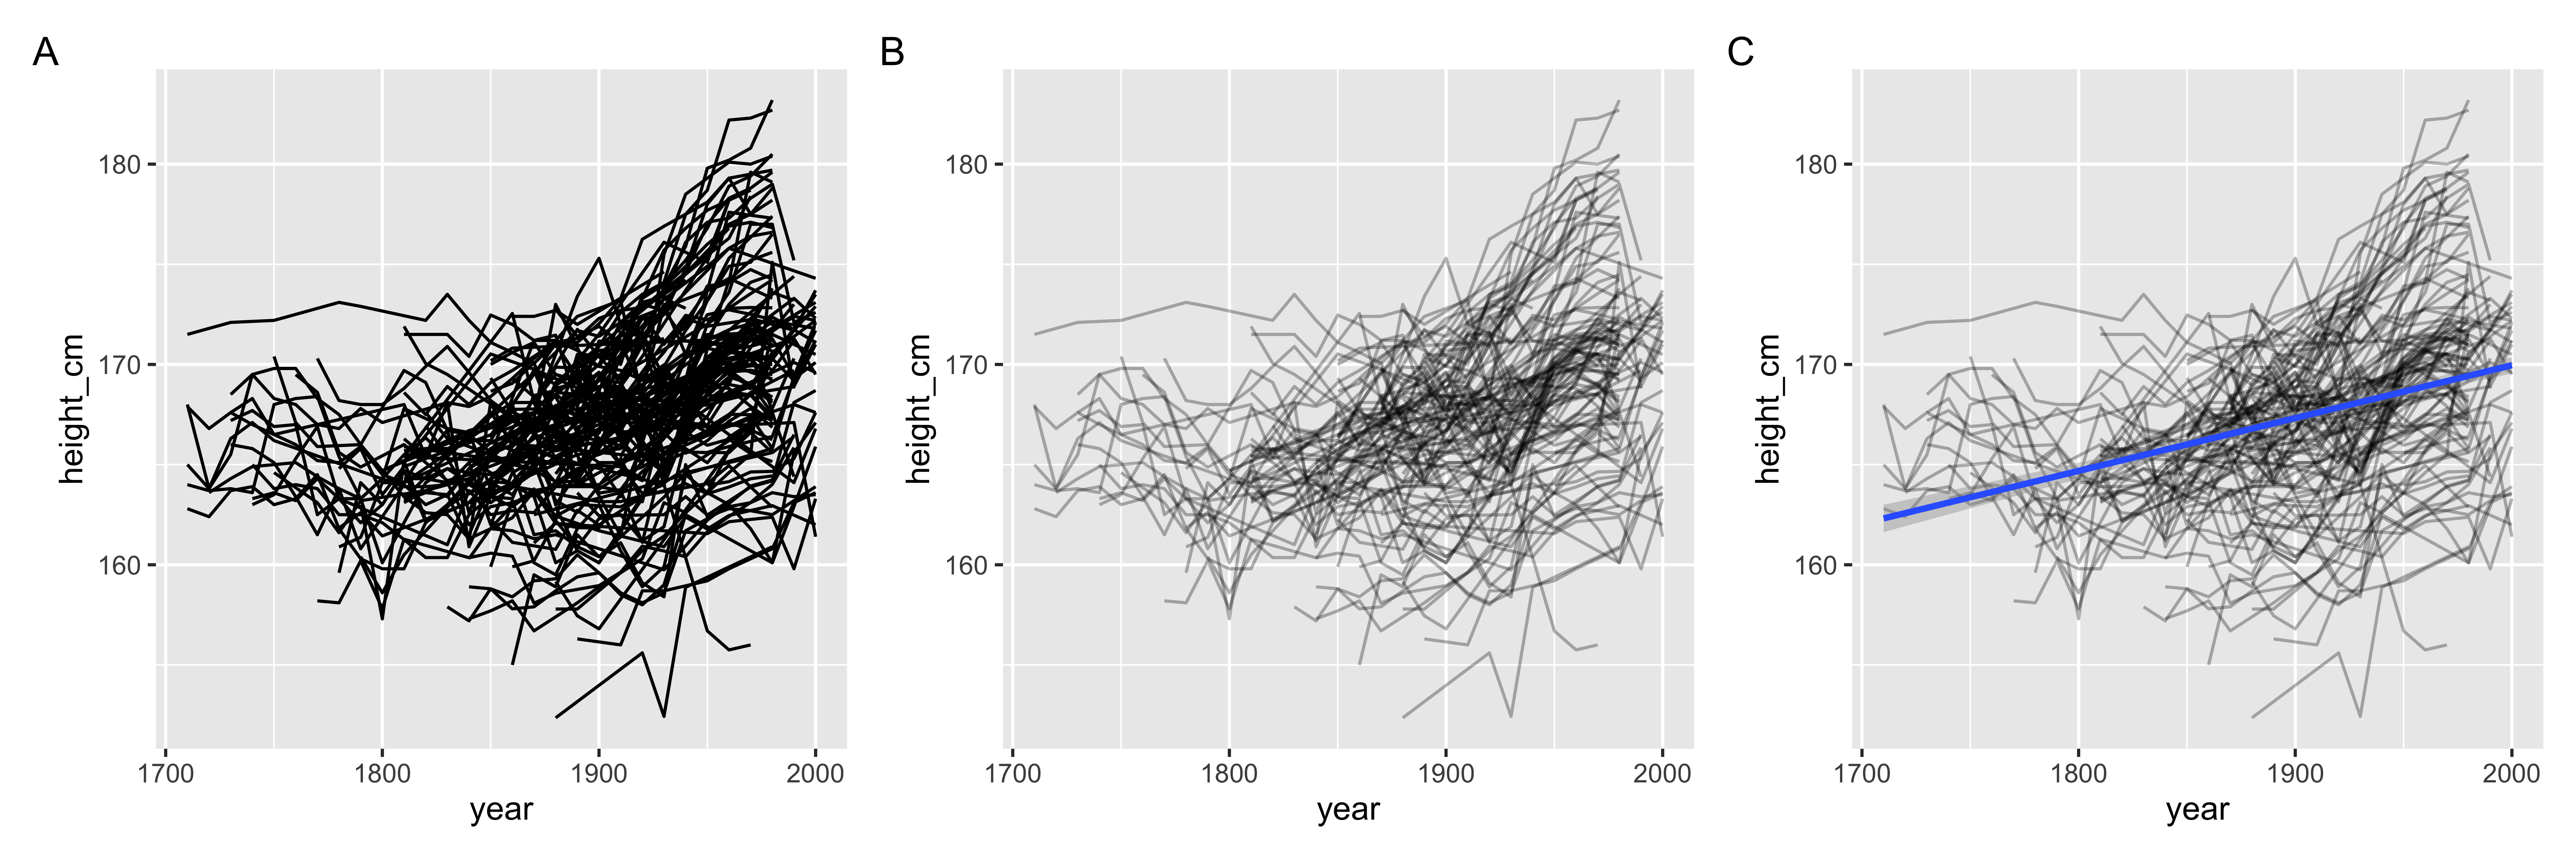
\includegraphics[width=0.95\linewidth]{brolgar-paper_files/figure-latex/spaghetti-1} 

}

\caption{The full dataset shown as a spaghetti plot (A), with transparency (B), and with a linear model overlayed (C). It is still hard to see the individuals.}\label{fig:spaghetti}
\end{figure}

This paper demonstrates how to effectively and efficiently explore longitudinal data, using the R package, \CRANpkg{brolgar}. We examine four problems in exploring longitudinal data:

\begin{enumerate}
\def\labelenumi{\arabic{enumi}.}
\tightlist
\item
  How to sample the data
\item
  Finding interesting individuals
\item
  Finding representative individuals
\item
  Understanding a model
\end{enumerate}

This paper proceeds in the following way: first, a brief review of existing approaches to longitudinal data, then the definition of longitudinal data, then approaches to these four problems are discussed, followed by a summary.

\hypertarget{background}{%
\section{Background}\label{background}}

R provides basic time series, \CRANpkg{ts}, objects, which are vectors or matrices that represent data sampled at equally spaced points in time. These have been extended through packages such as \CRANpkg{xts}, and \CRANpkg{zoo} (Ryan and Ulrich 2020; Zeileis and Grothendieck 2005), which only consider data in a wide format with a regular implied time series. These are not appropriate for longitudinal data, which can have indexes that are not time unit oriented, such as ``Wave 1\ldots n'', or may contain irregular intervals.

Other packages focus more directly on panel data in R, focussing on data operations and model interfaces. The \CRANpkg{pmdplyr} package provides ``Panel Manoeuvres'' in \CRANpkg{dplyr}(Huntington-Klein and Khor 2020). It defines the data structure in as a \texttt{pibble} object (\textbf{p}anel t\textbf{ibble}), requiring an \texttt{id} and \texttt{group} column being defined to identify the unique identifier and grouping. The \CRANpkg{pmdplyr} package focuses on efficient and custom joins and functions, such as \texttt{inexact\_left\_join()}. It does not implement tidyverse equivalent tools, but instead extends their usecase with a new function, for example \texttt{mutate\_cascade} and \texttt{mutate\_subset}. The \CRANpkg{panelr} package provides an interface for data reshaping on panel data, providing widening and lengthening functions (\texttt{widen\_panel()} and \texttt{long\_panel()} (Long 2020)). It also provides model facilitating functions by providing its own interface for mixed effects models. The \CRANpkg{plm} package (Millo 2017) for panel data econometrics provides methods for estimating models such as GMM for panel data, and testing, for example for model specification or serial correlation. It also provides a data structure, the \texttt{pdata.frame}, which stores the index attribute of the individual and time dimensions, for use within the package's functions.

These software generally re-implement their own custom panel data class object, as well as custom data cleaning tasks, such as reshaping into long and wide form. They all share similar features, providing some identifying or index variable, and some grouping or key.

\hypertarget{longitudinal-data-structures}{%
\section{Longitudinal Data Structures}\label{longitudinal-data-structures}}

Longitudinal data is a sibling of many other temporal data forms, including panel data, repeated measures, and time series. The differences are many, and can be in data collection, context and even the field of research. Time series are usually long and regularly spaced in time. Panel data may measure different units at each time point and aggregate these values by a categorical or key variable. Repeated measures typically measure before and after treatment effects. We like to think of longitudinal as measuring the same individual (e.g.~wage earner) over time, but this definition is not universally agreed on. Despite the differences, they all share a fundamental similarity: they are measurements over a time period.

This time period has structure - the time component (dates, times, waves, seconds, etc), and the spacing between measurements - unequal or equal. This data structure needs to be respected during analysis to preserve the lowest level of granularity, to avoid for example, collapsing across month when the data is collected every second, or assuming measurements occur at fixed time intervals. These mistakes can be avoided by encoding the data structure into the data itself. This information can then be accessed by analysis tools, providing a consistent way to understand and summarise the data. This ensures the different types of longitudinal data previously mentioned can be handled in the same way.

\hypertarget{building-on-a-tsibble}{%
\subsection{Building on a tsibble}\label{building-on-a-tsibble}}

Since longitudinal data can be thought of as ``individuals repeatedly measured through time'', they can be considered as a type of time series, as defined in Hyndman and Athanasopoulos (2018): ``Anything that is observed sequentially over time \textbf{is a time series}''. This definition has been realised as a time series \texttt{tsibble} in (Wang, Cook, and Hyndman 2020). These objects are defined as data meeting these conditions:

\begin{enumerate}
\def\labelenumi{\arabic{enumi}.}
\tightlist
\item
  The \texttt{index}: the time variable
\item
  The \texttt{key}: variable(s) defining individual groups (or series)
\item
  The \texttt{index} and \texttt{key} (1 + 2) together determine a distinct row
\end{enumerate}

If the specified key and index pair do not define a distinct row - for example, if there are duplicates in the data, the \texttt{tsibble} will not be created. This helps ensure the data is properly understood and cleaned before analysis is conducted, removing avoidable errors that might have impacted downstream decisions.

We can formally define our \texttt{heights} data from Figure \ref{fig:heights-sample-plot} as a \texttt{tsibble} using, \texttt{as\_tsibble}:

\begin{verbatim}
heights_brolgar <- as_tsibble(heights_brolgar,
                      index = year,
                      key = country,
                      regular = FALSE)
\end{verbatim}

The \texttt{index} is \texttt{year}, the \texttt{key} is \texttt{country}, and \texttt{regular\ =\ FALSE} since the intervals in the years measured are not regular. Using a \texttt{tsibble} means that the index and key time series information is recorded only \textbf{once}, and can be referred to many times in other parts of the data analysis by time-aware tools.

In addition to providing consistent ways to manipulate time series data, further benefits to building on \CRANpkg{tsibble} are how it works within the \texttt{tidyverse} ecosystem, as well as the tidy time series packages called ``tidyver\textbf{ts}'', containing \CRANpkg{fable} (O'Hara-Wild, Hyndman, and Wang 2020a), \CRANpkg{feasts}, (O'Hara-Wild, Hyndman, and Wang 2020b). For example, \CRANpkg{tsibble} provides modified \texttt{tidyverse} functions to explore implicit missing values in the \texttt{index} (e.g., \texttt{has\_gaps()} and \texttt{fill\_gaps()}), as well as grouping and partitioning based on the index with \texttt{index\_by()}. For full details and examples of use with the tidyverts time series packages, see Wang, Cook, and Hyndman (2020).

The \CRANpkg{brolgar} package uses \CRANpkg{tsibble} so users can take advantage of these tools, learning one way of operating a data analysis that will work and have overlap with other contexts.

\hypertarget{characterising-individual-series}{%
\subsection{Characterising Individual Series}\label{characterising-individual-series}}

\hypertarget{calculating-a-feature}{%
\subsubsection{Calculating a feature}\label{calculating-a-feature}}

We can summarise the individual series by collapsing their many measurements into a single statistic, such as the minimum, maximum, or median, with one row per key. We do this with the \texttt{features} function from the \CRANpkg{fabletools} package, made available in \CRANpkg{brolgar}. This provides a summary of a given variable, accounting for the time series structure, and returning one row per key specified. It can be thought of as a time-series aware variant of the \texttt{summarise} function from \CRANpkg{dplyr}. The \texttt{feature} function works by specifying the data, the variable to summarise, and the feature to calculate. A template is shown below

\begin{verbatim}
features(<DATA>, <VARIABLE>, <FEATURE>)
\end{verbatim}

or, with the pipe:

\begin{verbatim}
<DATA> %>% features(<VARIABLE>, <FEATURE>)
\end{verbatim}

For example, to calculate the minimum height for each key (country), in \texttt{heights}, we specify the \texttt{heights} data, then the variable to calculate features on, \texttt{height\_cm}, then the feature to calculate, \texttt{min} (we write \texttt{c(min\ =\ min)} so the column calculated gets the name ``min''):

\begin{verbatim}
heights_min <- features(.tbl = heights_brolgar, 
                        .var = height_cm, 
                        features = c(min = min))

heights_min
\end{verbatim}

\begin{verbatim}
#> # A tibble: 119 x 2
#>    country       min
#>    <chr>       <dbl>
#>  1 Afghanistan  161.
#>  2 Algeria      166.
#>  3 Angola       159.
#>  4 Argentina    167.
#>  5 Armenia      164.
#>  6 Australia    170 
#>  7 Austria      162.
#>  8 Azerbaijan   170.
#>  9 Bangladesh   160.
#> 10 Belgium      163.
#> # ... with 109 more rows
\end{verbatim}

We call these summaries \texttt{features} of the data. We can use this information to summarise these features of the data, for example, visualising the distribution of minimum values (Figure \ref{fig:feature-min-med-max}A).

We are not limited to one feature at a time, many features can also be calculated, for example:

\begin{verbatim}
heights_three <- heights_brolgar %>%
  features(height_cm, c(
    min = min,
    median = median,
    max = max
  ))

heights_three
\end{verbatim}

\begin{verbatim}
#> # A tibble: 119 x 4
#>    country       min median   max
#>    <chr>       <dbl>  <dbl> <dbl>
#>  1 Afghanistan  161.   167.  168.
#>  2 Algeria      166.   169   171.
#>  3 Angola       159.   167.  169.
#>  4 Argentina    167.   168.  174.
#>  5 Armenia      164.   169.  172.
#>  6 Australia    170    172.  178.
#>  7 Austria      162.   167.  179.
#>  8 Azerbaijan   170.   172.  172.
#>  9 Bangladesh   160.   162.  164.
#> 10 Belgium      163.   166.  177.
#> # ... with 109 more rows
\end{verbatim}

These can then be visualised together (Figure \ref{fig:feature-min-med-max}).

\begin{figure}

{\centering 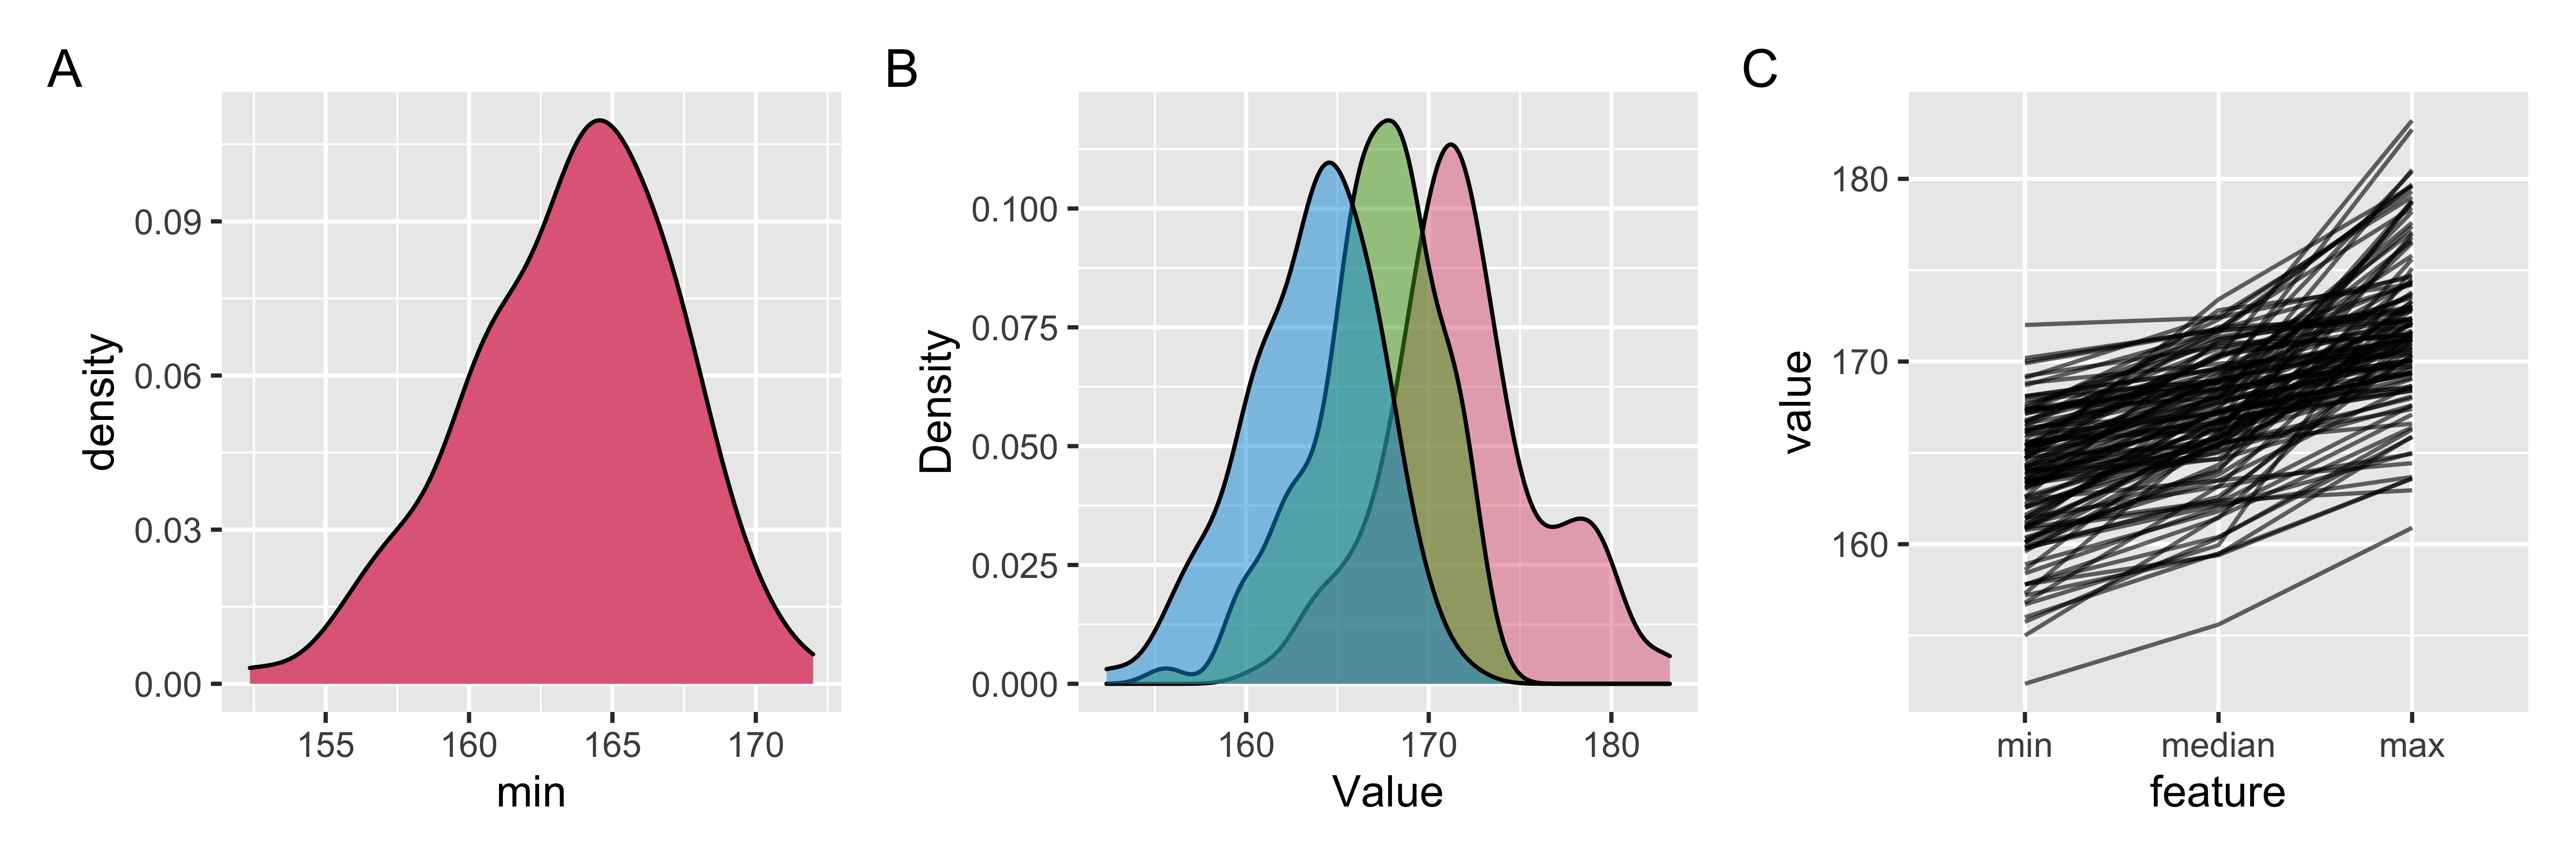
\includegraphics[width=0.95\linewidth]{brolgar-paper_files/figure-latex/feature-min-med-max-1} 

}

\caption{Three plots showing the distribution of minimum, median, and maximum values of height in centimeters. Part A shows just the distribution of minimum, part B shows the distribution of minimum, median, and maximum, and part C shows these three values plotted together as a line graph. We see that there is overlap amongst all three statistics. That is, some countries minimum heights are taller than some countries maximum heights.}\label{fig:feature-min-med-max}
\end{figure}

These sets of features can be pre-specified, for example, \texttt{brolgar} provides a five number summary (minimum, 25th quantile, median, mean, 75th quantile, and maximum) of the data with \texttt{feat\_five\_num}:

\begin{verbatim}
heights_five <- heights_brolgar %>%
  features(height_cm, feat_five_num)

heights_five
\end{verbatim}

\begin{verbatim}
#> # A tibble: 119 x 6
#>    country       min   q25   med   q75   max
#>    <chr>       <dbl> <dbl> <dbl> <dbl> <dbl>
#>  1 Afghanistan  161.  164.  167.  168.  168.
#>  2 Algeria      166.  168.  169   170.  171.
#>  3 Angola       159.  160.  167.  168.  169.
#>  4 Argentina    167.  168.  168.  170.  174.
#>  5 Armenia      164.  166.  169.  172.  172.
#>  6 Australia    170   171.  172.  173.  178.
#>  7 Austria      162.  164.  167.  169.  179.
#>  8 Azerbaijan   170.  171.  172.  172.  172.
#>  9 Bangladesh   160.  162.  162.  163.  164.
#> 10 Belgium      163.  164.  166.  168.  177.
#> # ... with 109 more rows
\end{verbatim}

This takes the \texttt{heights} data, pipes it to \texttt{features}, and then instructs it to summarise the \texttt{height\_cm} variable, using \texttt{feat\_five\_num}. There are several handy functions for calculating features of the data that
\texttt{brolgar} provides. These all start with \texttt{feat\_}, and include:

\begin{itemize}
\tightlist
\item
  \texttt{feat\_ranges()}: min, max, range difference, interquartile range;
\item
  \texttt{feat\_spread()}: variance, standard deviation, median absolute distance, and interquartile range;
\item
  \texttt{feat\_monotonic()}: is it always increasing, decreasing, or unvarying?;
\item
  \texttt{feat\_diff\_summary()}: the summary statistics of the differences amongst a value, including the five number summary, as well as the standard deviation and variance;
\item
  \texttt{feat\_brolgar()}, which will calculate all features available in the \CRANpkg{brolgar} package.
\item
  Other examples of features from the \CRANpkg{feasts} package.
\end{itemize}

\hypertarget{feature-sets}{%
\subsubsection{Feature sets}\label{feature-sets}}

If you want to run many or all features from a package on your data you can collect them all with \texttt{feature\_set}. For example:

\begin{verbatim}
library(fabletools)
feat_set_brolgar <- feature_set(pkgs = "brolgar")
length(feat_set_brolgar)
\end{verbatim}

\begin{verbatim}
#> [1] 6
\end{verbatim}

You could then run these like so:

\begin{verbatim}
heights_brolgar %>%
  features(height_cm, feat_set_brolgar)
\end{verbatim}

\begin{verbatim}
#> # A tibble: 119 x 46
#>    country     min...1 med...2 max...3 min...4 q25...5 med...6 q75...7 max...8
#>    <chr>         <dbl>   <dbl>   <dbl>   <dbl>   <dbl>   <dbl>   <dbl>   <dbl>
#>  1 Afghanistan    161.    167.    168.    161.    164.    167.    168.    168.
#>  2 Algeria        166.    169     171.    166.    168.    169     170.    171.
#>  3 Angola         159.    167.    169.    159.    160.    167.    168.    169.
#>  4 Argentina      167.    168.    174.    167.    168.    168.    170.    174.
#>  5 Armenia        164.    169.    172.    164.    166.    169.    172.    172.
#>  6 Australia      170     172.    178.    170     171.    172.    173.    178.
#>  7 Austria        162.    167.    179.    162.    164.    167.    169.    179.
#>  8 Azerbaijan     170.    172.    172.    170.    171.    172.    172.    172.
#>  9 Bangladesh     160.    162.    164.    160.    162.    162.    163.    164.
#> 10 Belgium        163.    166.    177.    163.    164.    166.    168.    177.
#> # ... with 109 more rows, and 37 more variables: min...9 <dbl>, max...10 <dbl>,
#> #   range_diff...11 <dbl>, iqr...12 <dbl>, var...13 <dbl>, sd...14 <dbl>,
#> #   mad...15 <dbl>, iqr...16 <dbl>, min...17 <dbl>, max...18 <dbl>,
#> #   median <dbl>, mean <dbl>, q25...21 <dbl>, q75...22 <dbl>, range1 <dbl>,
#> #   range2 <dbl>, range_diff...25 <dbl>, sd...26 <dbl>, var...27 <dbl>,
#> #   mad...28 <dbl>, iqr...29 <dbl>, increase...30 <dbl>, decrease...31 <dbl>,
#> #   unvary...32 <dbl>, diff_min <dbl>, diff_q25 <dbl>, diff_median <dbl>, ...
\end{verbatim}

To see other features available in the \CRANpkg{feasts} R package run \texttt{library(feasts)} then \texttt{?fabletools::feature\_set}.

\hypertarget{creating-your-own-feature}{%
\subsubsection{Creating your own feature}\label{creating-your-own-feature}}

To create your own features or summaries to pass to \texttt{features}, you provide a named vector of functions. These can include functions that you have written yourself. For example, returning the first three elements of a series, by writing our own \texttt{second} and \texttt{third} functions.

\begin{verbatim}
second <- function(x) nth(x, n = 2)
third <- function(x) nth(x, n = 3)

feat_first_three <- c(first = first,
                      second = second,
                      third = third)
\end{verbatim}

These are then passed to \texttt{features} like so:

\begin{verbatim}
heights_brolgar %>%
  features(height_cm, feat_first_three)
\end{verbatim}

\begin{verbatim}
#> # A tibble: 119 x 4
#>    country     first second third
#>    <chr>       <dbl>  <dbl> <dbl>
#>  1 Afghanistan  168.   166.  167.
#>  2 Algeria      169.   166.  169 
#>  3 Angola       160.   159.  160.
#>  4 Argentina    170.   168.  168 
#>  5 Armenia      169.   168.  166.
#>  6 Australia    170    171.  170.
#>  7 Austria      165.   163.  162.
#>  8 Azerbaijan   170.   171.  171.
#>  9 Bangladesh   162.   162.  164.
#> 10 Belgium      163.   164.  164 
#> # ... with 109 more rows
\end{verbatim}

As well, \texttt{brolgar} provides some useful additional features for the five number summary, \texttt{feat\_five\_num}, whether keys are monotonically increasing \texttt{feat\_monotonic}, and measures of spread or variation, \texttt{feat\_spread}. Inside \texttt{brolgar}, the features are created with the following syntax:

\begin{verbatim}
feat_five_num <- function(x, ...) {
  c(
    min = b_min(x, ...),
    q25 = b_q25(x, ...),
    med = b_median(x, ...),
    q75 = b_q75(x, ...),
    max = b_max(x, ...)
  )
}
\end{verbatim}

Here the functions \texttt{b\_} are functions with a default of \texttt{na.rm\ =\ TRUE}, and in
the cases of quantiles, they use \texttt{type\ =\ 8}, and \texttt{names\ =\ FALSE}. What is particularly useful is that these will work on any type of time series data, and you can use other more typical time series features from the \CRANpkg{feasts} package, such as autocorrelation, \texttt{feat\_acf()} and Seasonal and Trend decomposition using Loess \texttt{feat\_stl()} (O'Hara-Wild, Hyndman, and Wang 2020b).

This demonstrates a workflow that can be used to understand and explore your longitudinal data. The \CRANpkg{brolgar} package builds upon this workflow made available by \CRANpkg{feasts} and \CRANpkg{fabletools}. Users can also create their own features to summarise the data.

\hypertarget{breaking-up-the-spaghetti}{%
\section{Breaking up the Spaghetti}\label{breaking-up-the-spaghetti}}

Plots like Figure \ref{fig:spaghetti} are often called, ``spaghetti plots'', and can be useful for a high level understanding as a whole. However, we cannot process and understand the individuals when the data is presented like this.

\hypertarget{sampling}{%
\subsection{Sampling}\label{sampling}}

Just how spaghetti is portioned out for consumption, we can sample some of the data by randomly sampling the data into sub-plots with the \texttt{facet\_sample()} function (Figure \ref{fig:facet-sample}).

\begin{verbatim}
ggplot(heights_brolgar,
       aes(x = year,
           y = height_cm,
           group = country)) + 
  geom_line() + 
  facet_sample() + 
  scale_x_continuous(breaks = c(1750, 1850, 1950))
\end{verbatim}

\begin{figure}

{\centering 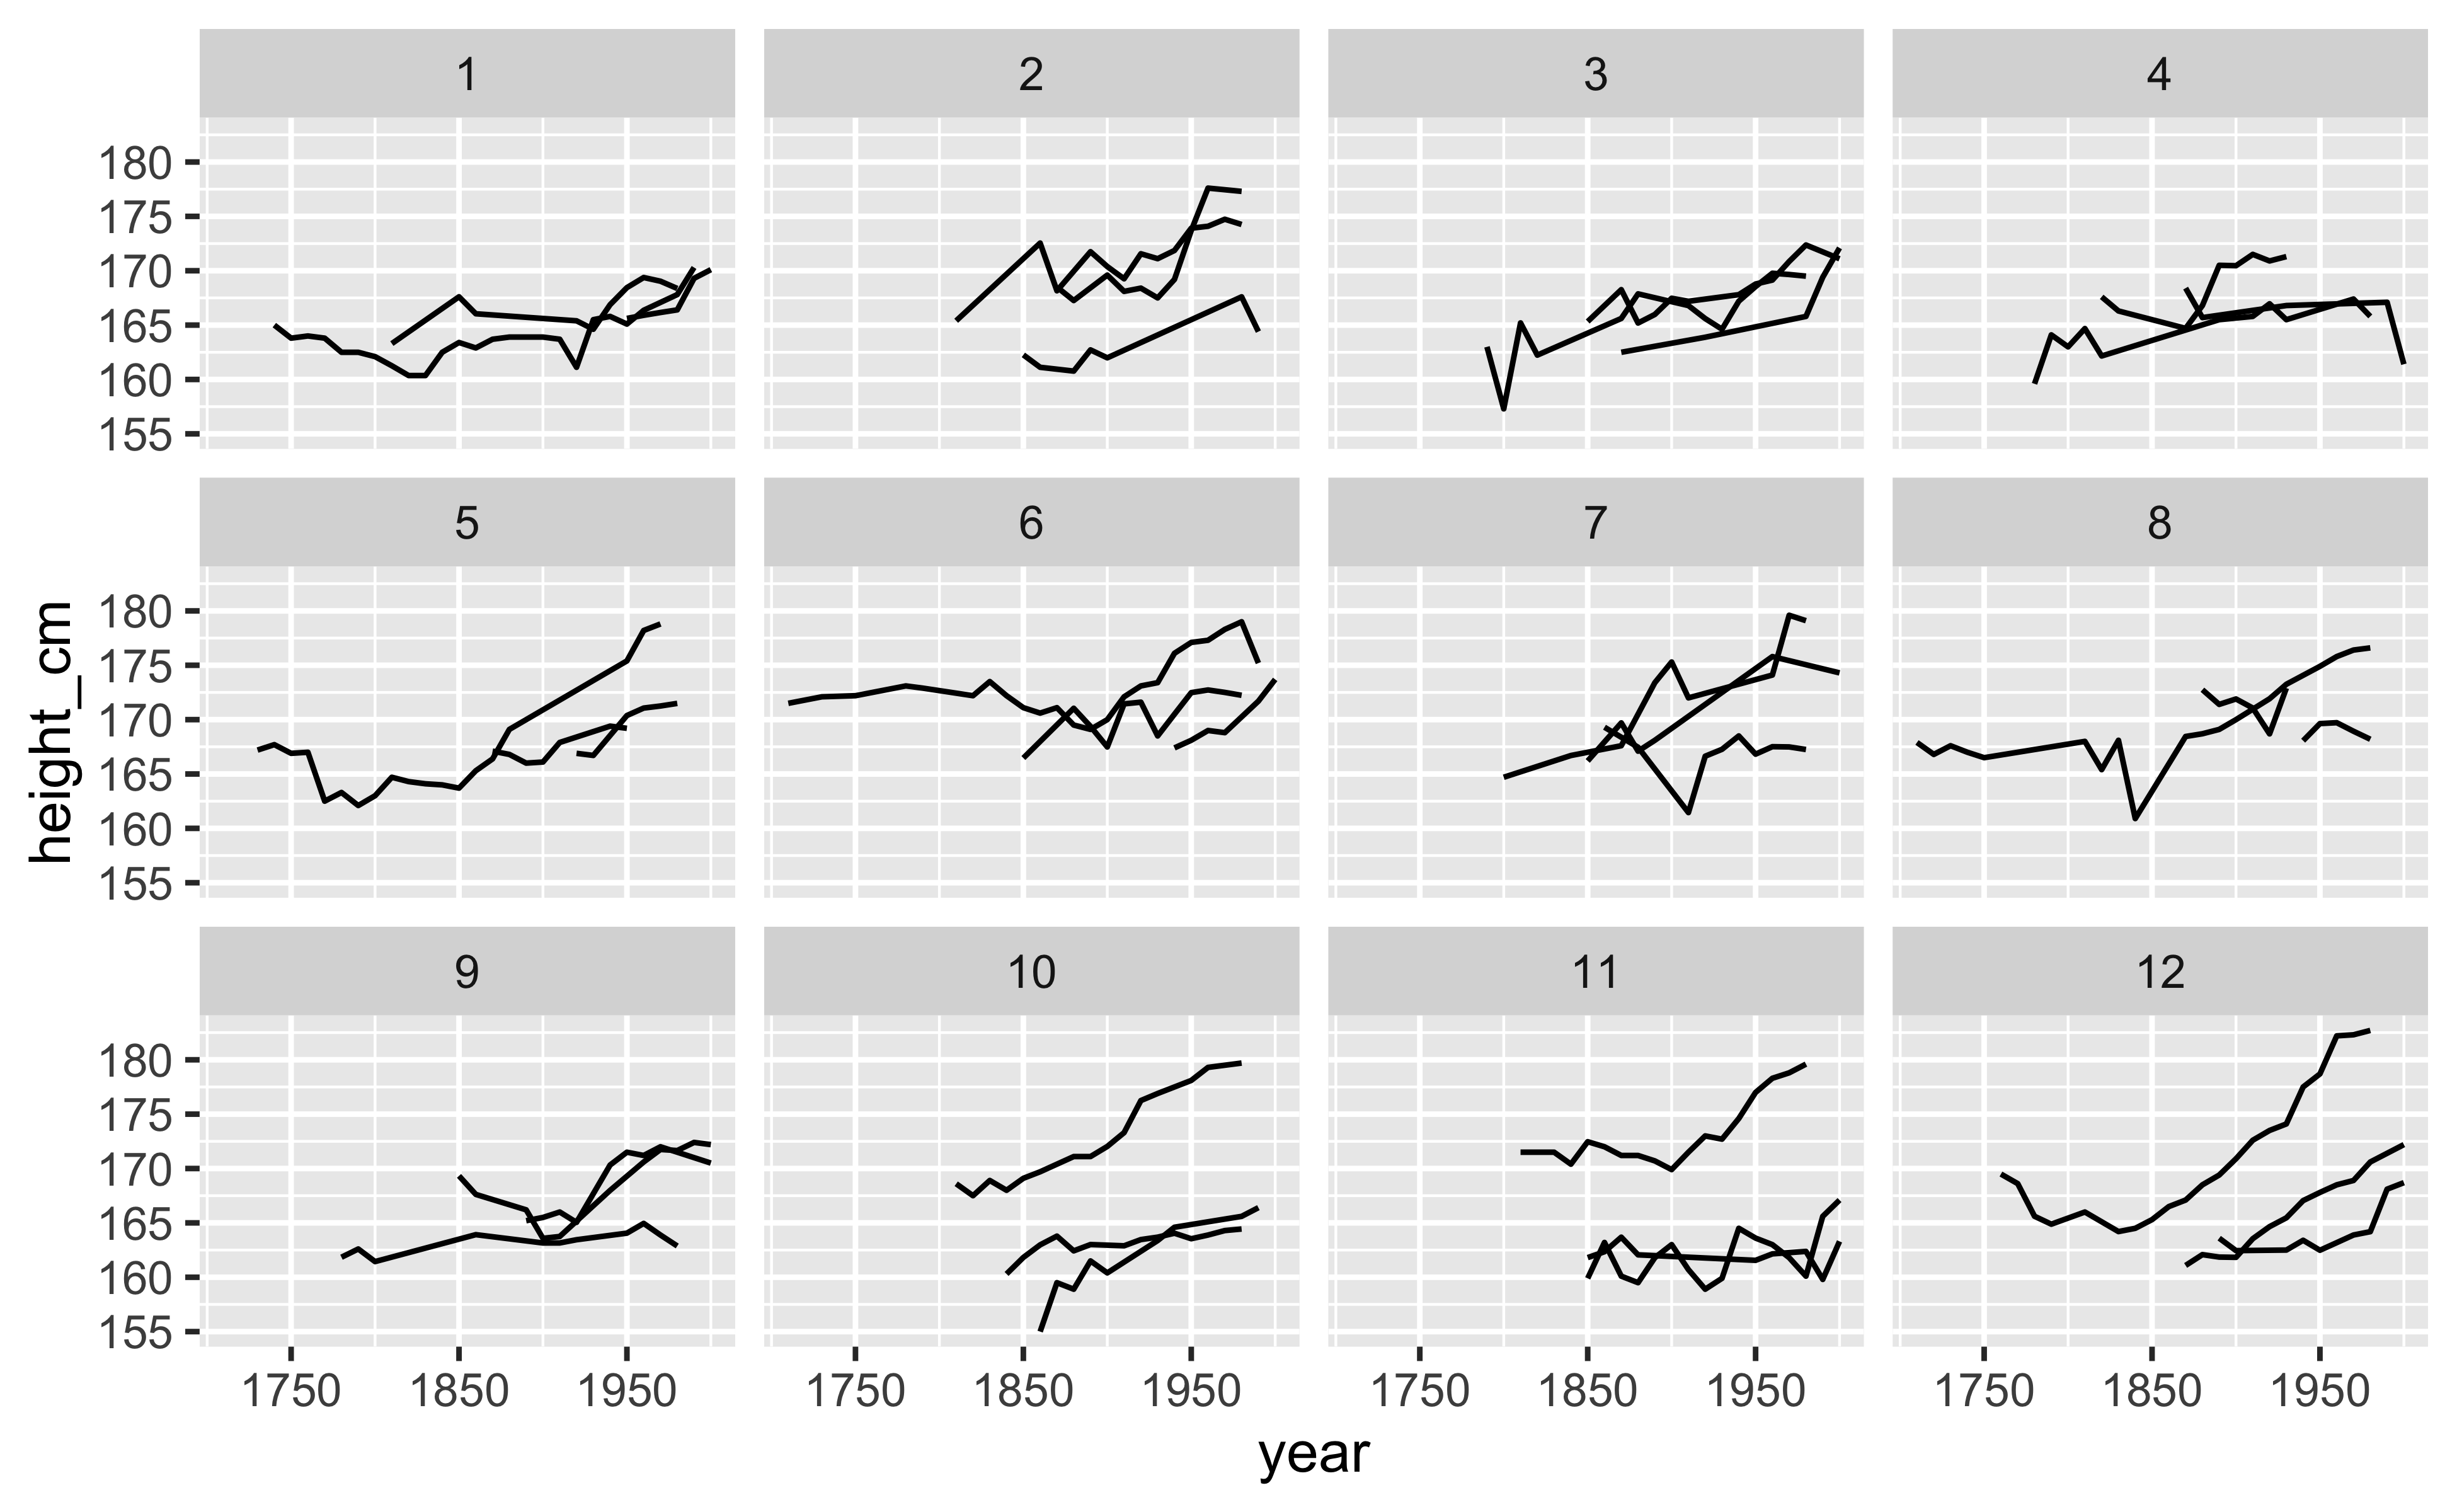
\includegraphics[width=0.95\linewidth]{brolgar-paper_files/figure-latex/facet-sample-1} 

}

\caption{Twelve facets with three keys per facet shown. This allows us to quickly view a random sample of the data.}\label{fig:facet-sample}
\end{figure}

This defaults to 12 facets and 3 samples per facet, and provides options for the number of facets, and the number of samples per facet. This means the user only needs to consider the most relevant questions: ``How many keys per facet?'' and ``How many facets to look at?''. The code to change the figure from Figure \ref{fig:spaghetti} into \ref{fig:facet-sample} requires only one line of code, shown below:

\begin{verbatim}
ggplot(heights_brolgar,
       aes(x = year,
           y = height_cm,
           group = country)) + 
  geom_line() + 
  facet_sample()
\end{verbatim}

\hypertarget{stratifying}{%
\subsection{Stratifying}\label{stratifying}}

Extending this idea of samples, we can instead look at \textbf{all} of the data, spread out equally over facets, using \texttt{facet\_strata()}. It uses 12 facets by default, controllable with \texttt{n\_strata}. The code to do so is shown below, creating Figure \ref{fig:facet-strata}.

\begin{verbatim}
ggplot(heights_brolgar,
       aes(x = year,
           y = height_cm,
           group = country)) + 
  geom_line() + 
  facet_strata() +
  scale_x_continuous(breaks = c(1750, 1850, 1950))
\end{verbatim}

\begin{figure}

{\centering 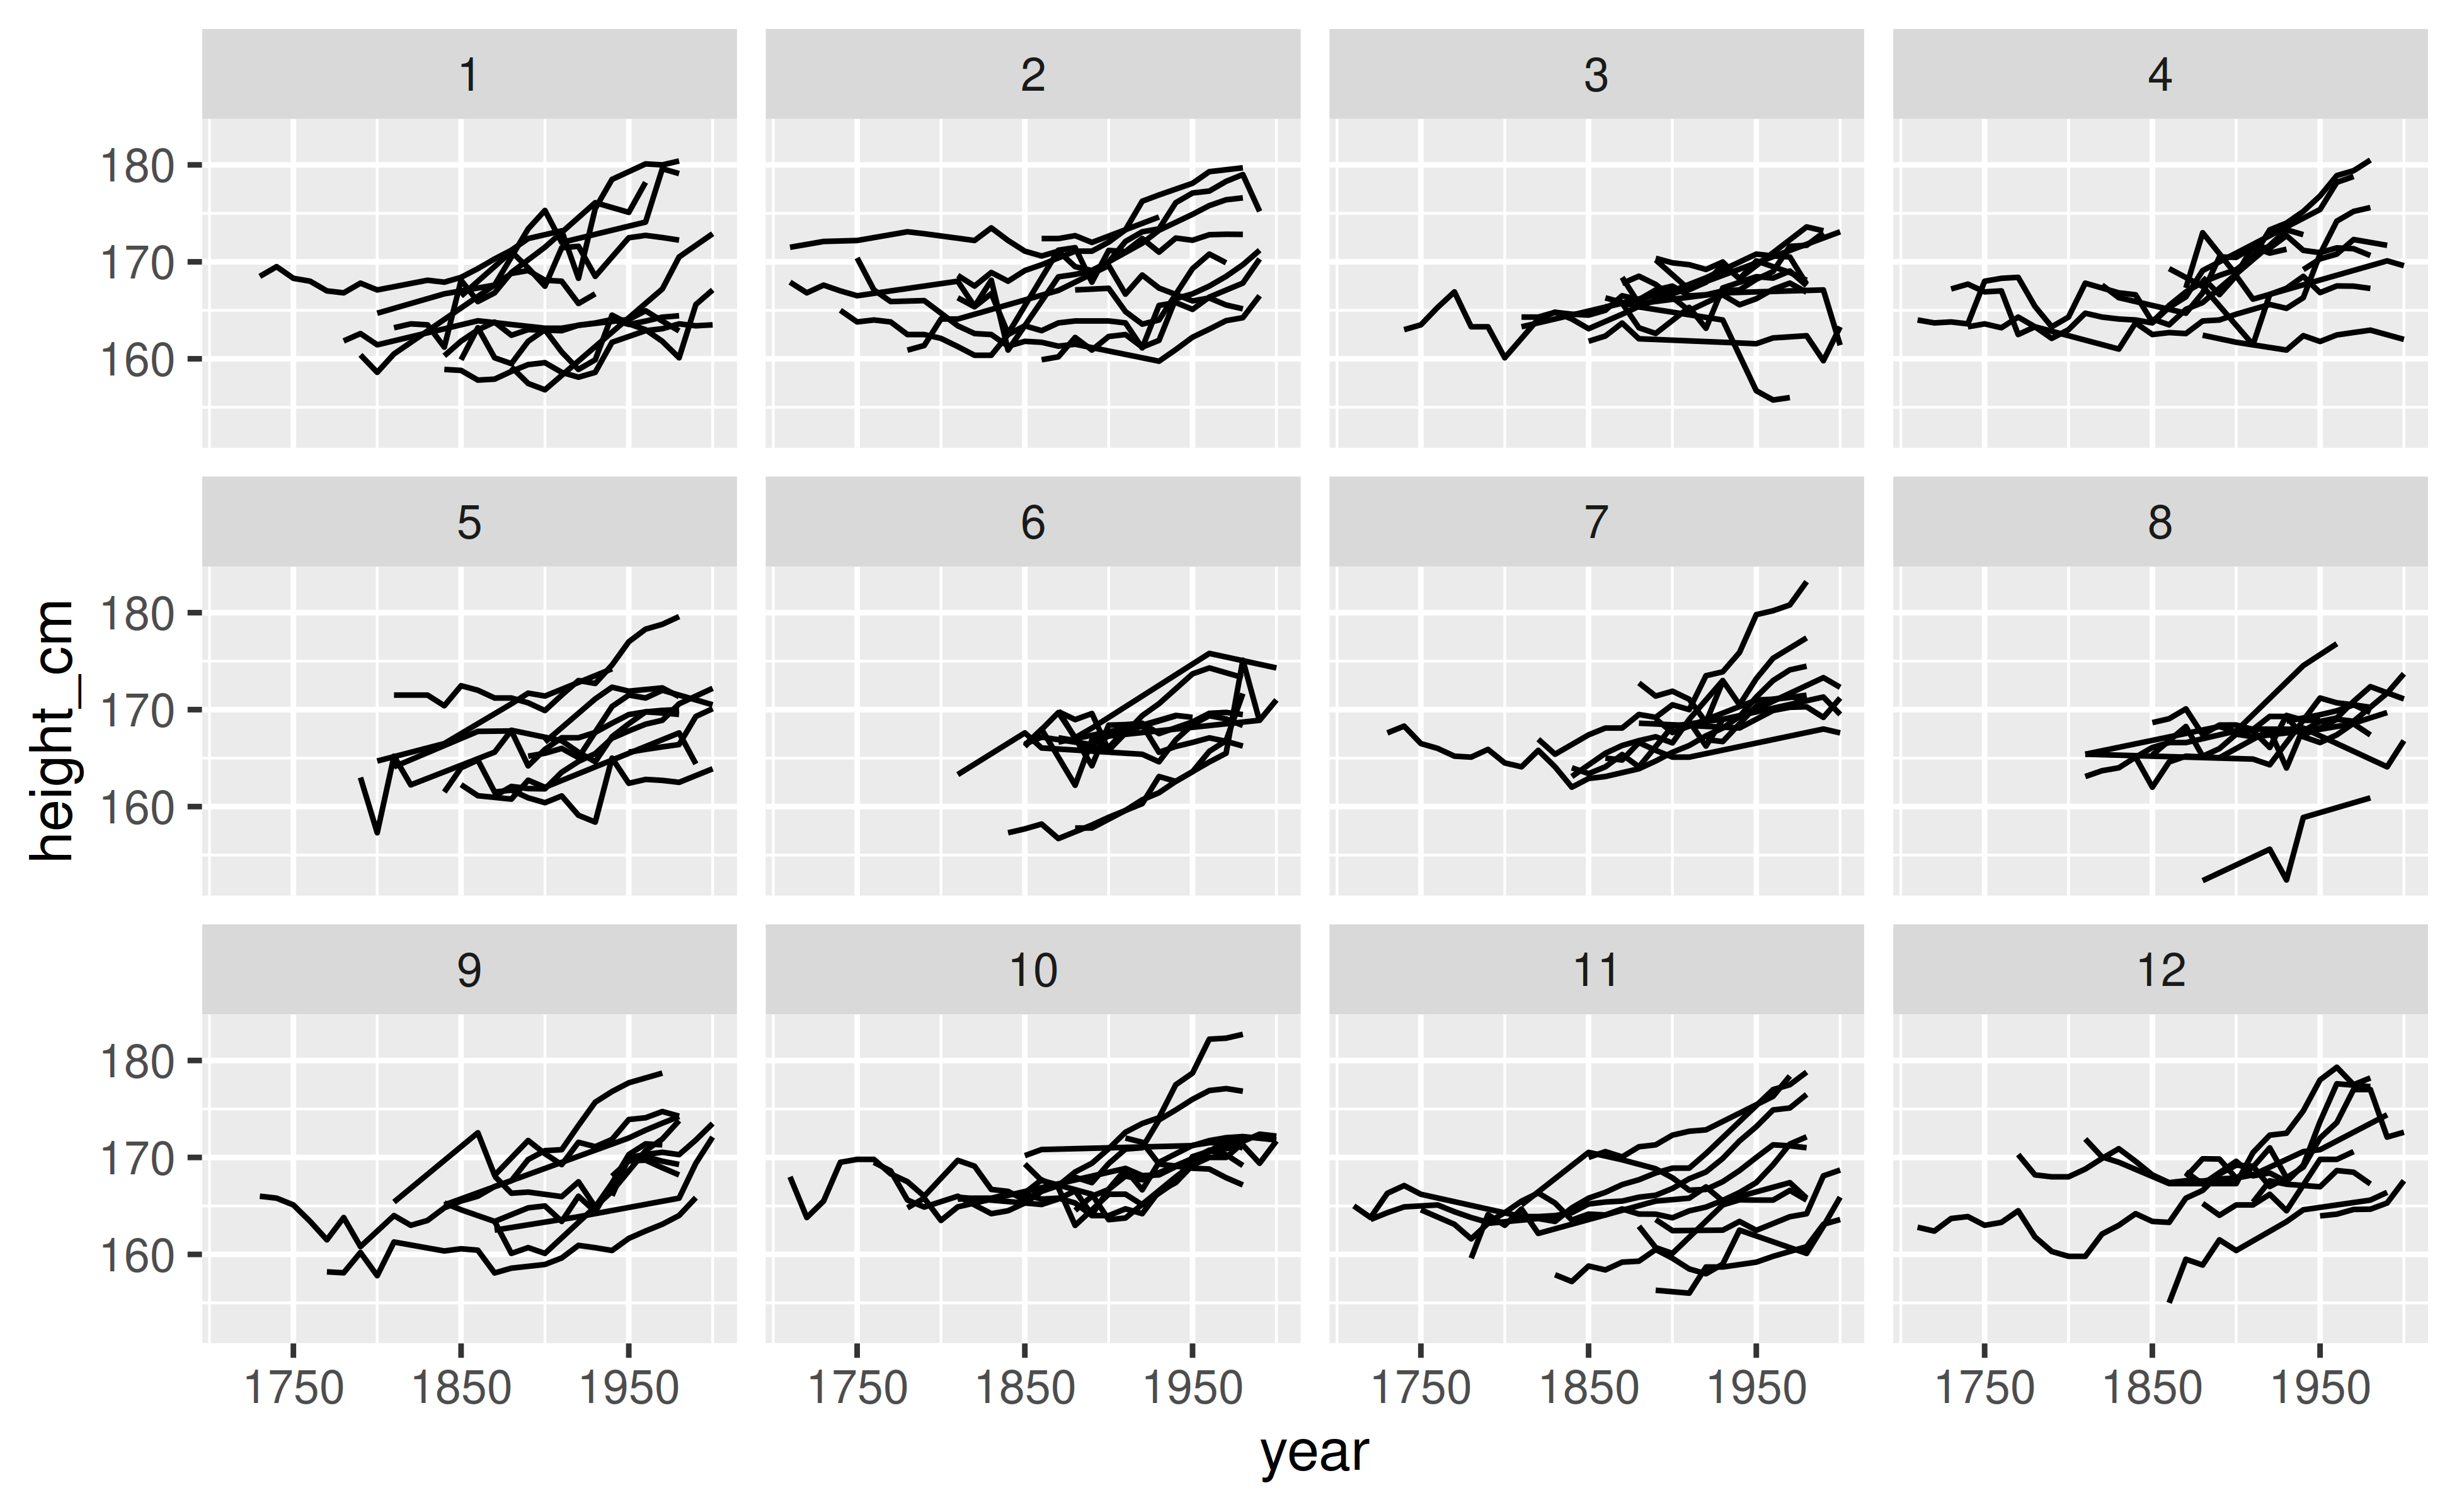
\includegraphics[width=0.95\linewidth]{brolgar-paper_files/figure-latex/facet-strata-1} 

}

\caption{All of the data is shown by spreading out each key across twelve facets. Each key is only shown once, and is randomly allocated to a facet.}\label{fig:facet-strata}
\end{figure}

\hypertarget{featuring}{%
\subsection{Featuring}\label{featuring}}

Figure \ref{fig:facet-sample} and Figure \ref{fig:facet-strata} only show each key once, being randomly assigned to a facet. We can meaningfully place the keys into facets, by arranging the heights ``along'' a variable, like \texttt{year}, using the \texttt{along} argument in \texttt{facet\_strata} to produce Figure \ref{fig:facet-year-along}:

\begin{verbatim}
ggplot(heights_brolgar,
       aes(x = year,
           y = height_cm,
           group = country)) + 
  geom_line() + 
  facet_strata(along = -year) + 
  scale_x_continuous(breaks = c(1750, 1850, 1950))
\end{verbatim}

\begin{figure}

{\centering 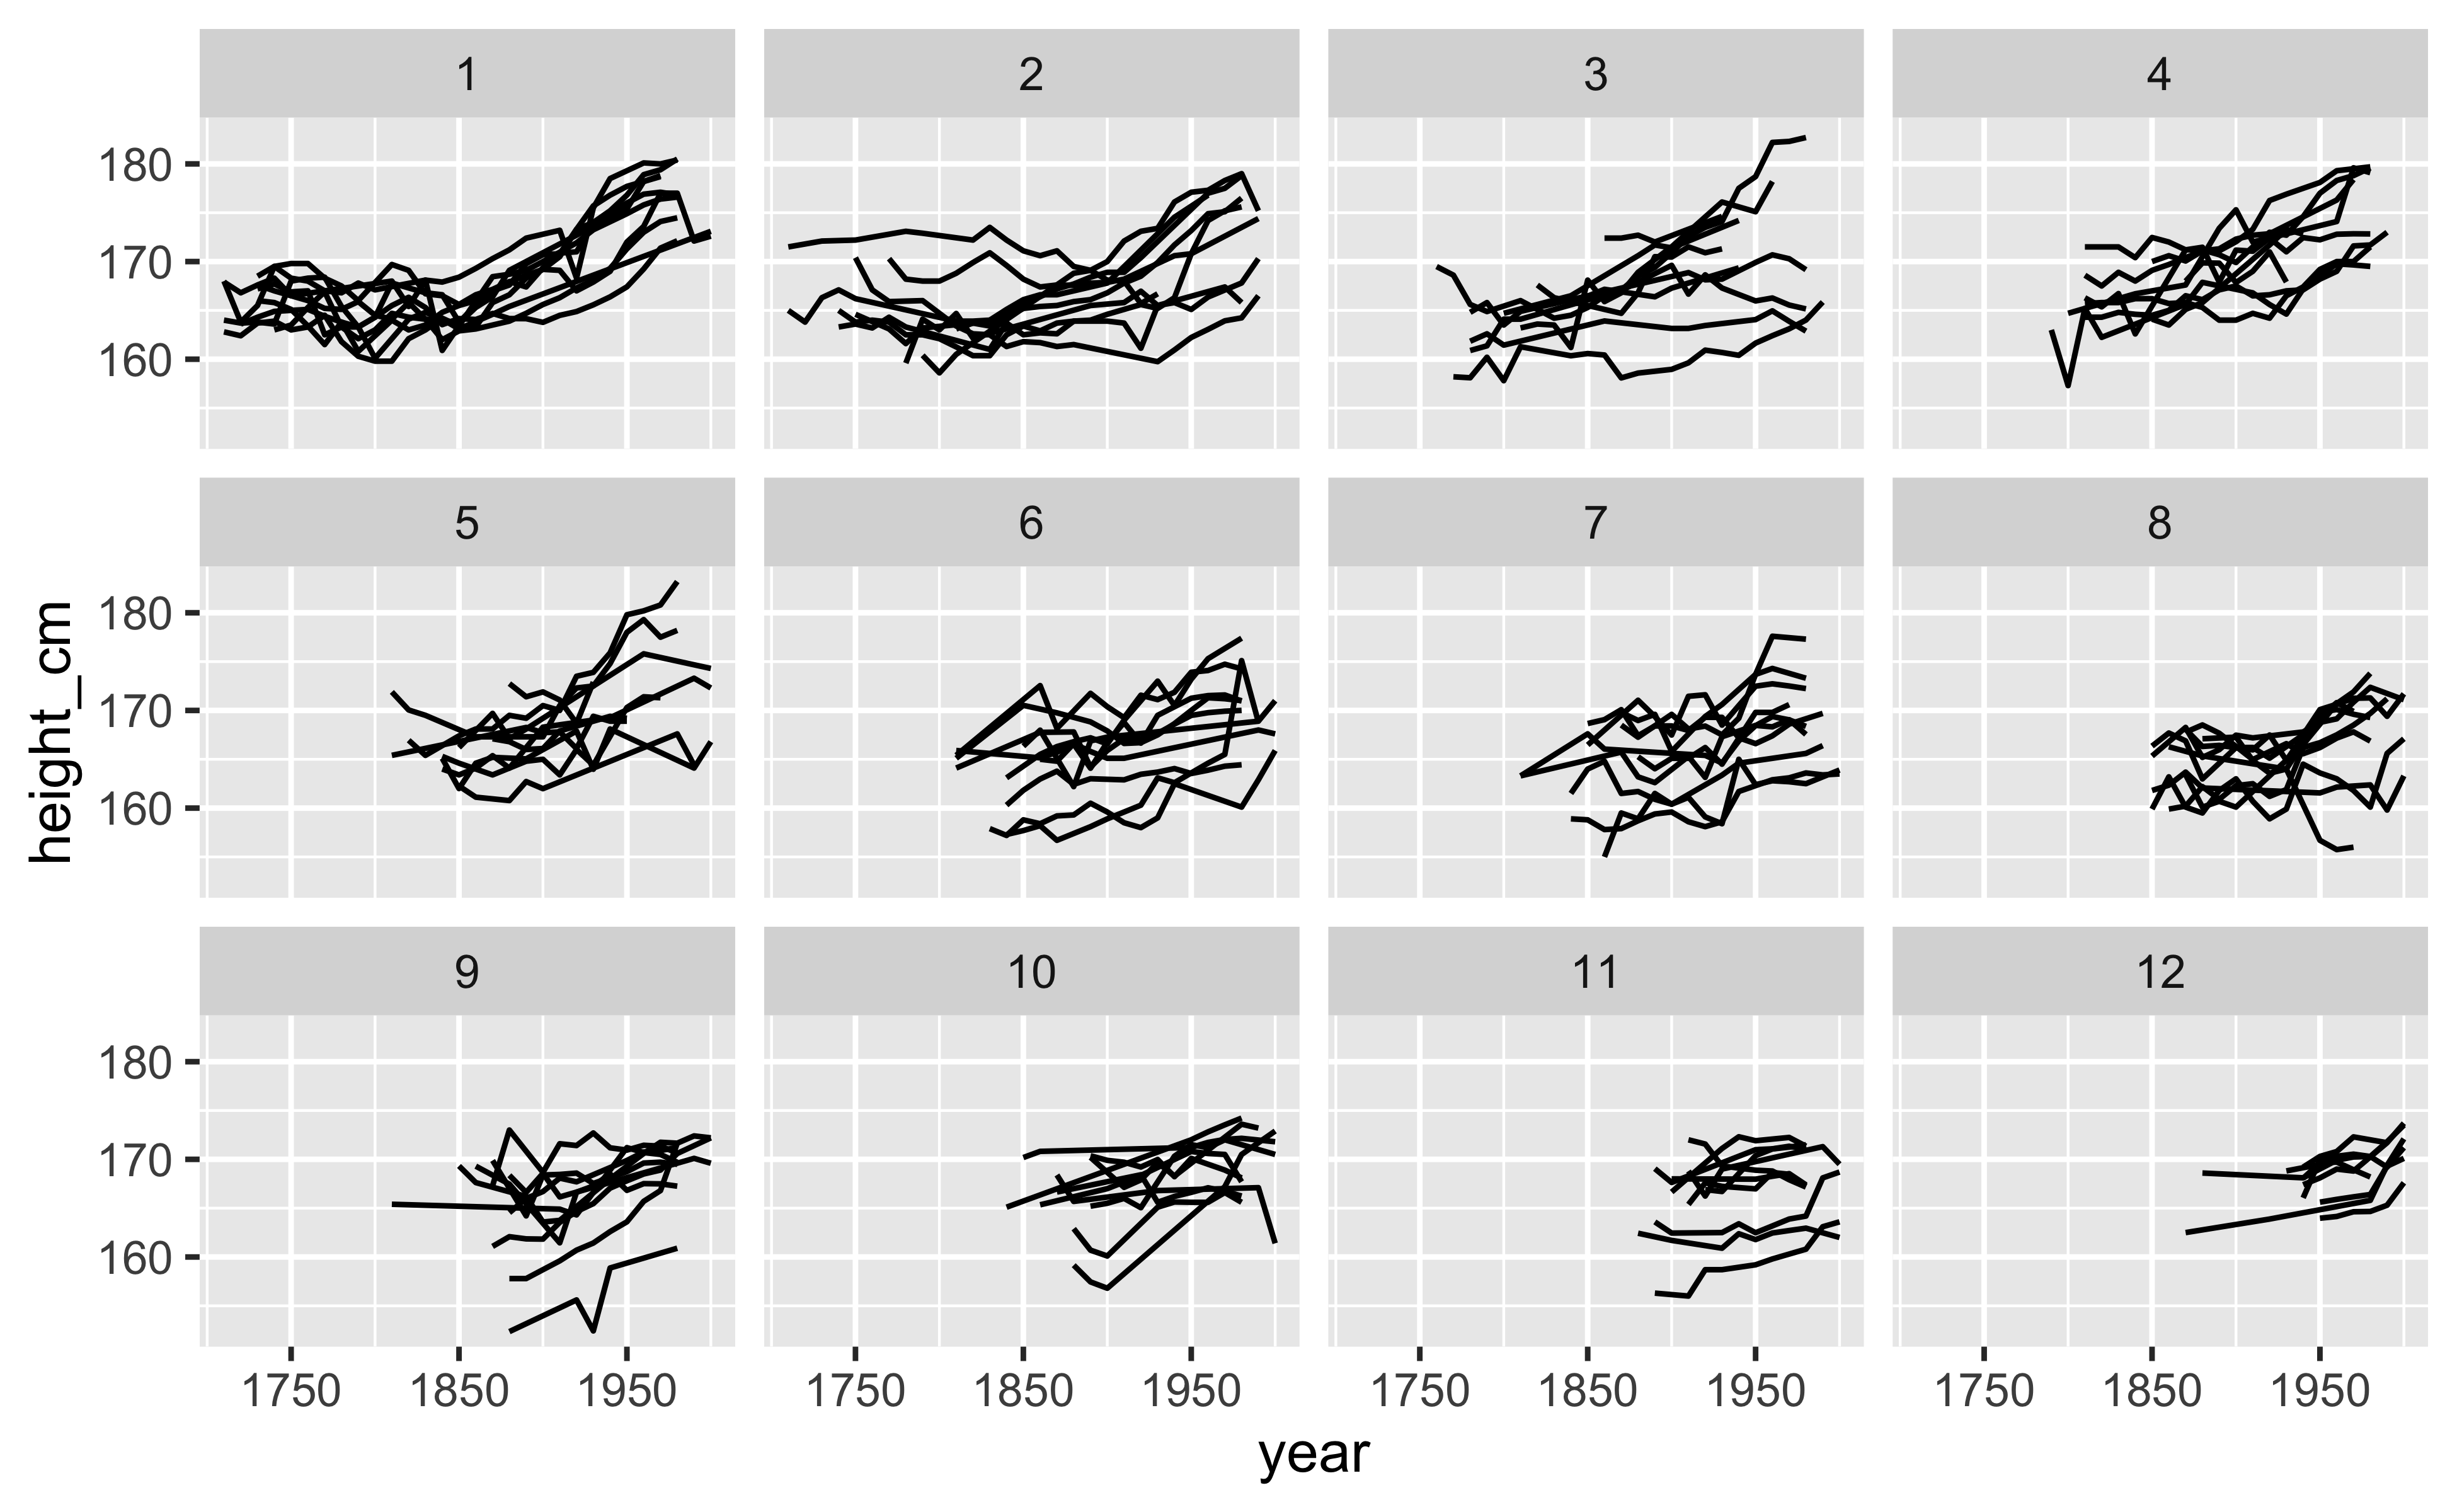
\includegraphics[width=0.95\linewidth]{brolgar-paper_files/figure-latex/facet-year-along-1} 

}

\caption{Displaying all the data across twelve facets. Instead of each key being randomly in a facet, each facet displays a specified range of values of year. In this case, the top left facet shows the keys with the earliest starting year, and the bottom right shows the facet with the latest starting year.}\label{fig:facet-year-along}
\end{figure}

We have not lost any of the data, only the order in which they are presented has changed. We learn the distribution and changes in heights over time, and those measured from the earliest times appear to be more similar, but there is much wider variation in the middle years, and then for more recent heights measured from the early 1900s, the heights are more similar. The starting point of each of these years seems to increase at roughly the same interval. This informs us that the starting times of the years is approximately uniform.

Together \texttt{facet\_sample()} and \texttt{facet\_strata()} allow for rapid exploration, by focusing on relevant questions instead of the minutiae. This is achieved by appropriately randomly assigning while maintaining key structure, keeping the correct number of keys per plot, and so on. For example, \texttt{facet\_sample()} the questions are: ``How many lines per facet'' and ``How many facets?'', and for \texttt{facet\_strata()} the questions are: ``How many facets / strata?'' and ``What to arrange plots along?''.

Answering these questions keeps the analysis in line with the analytic goals of exploring the data, rather than distracting to minutiae. This is a key theme of improving tools for data analysis. Abstracting away the parts that are not needed, so the analyst can focus on the task at hand.

Under the hood, \texttt{facet\_sample()} and \texttt{facet\_strata()} are powered with \texttt{sample\_n\_keys()} and \texttt{stratify\_keys()}. These can be used to create data structures used in \texttt{facet\_sample()} and \texttt{facet\_strata()}, and extend them for other purposes.

Using a \texttt{tsibble} stores important key and index components, in turn allowing for better ways to break up spaghetti plots so we can look at many and all sub-samples using \texttt{facet\_sample()} and \texttt{facet\_strata()}.

\hypertarget{book-keeping}{%
\section{Book-keeping}\label{book-keeping}}

Longitudinal data is not always measured at the same time and at the same frequency. When exploring longitudinal data, a useful first step is to explore the frequency of measurements of the index. We can check if the index is regular using \texttt{index\_regular()} and summarise the spacing of the index with \texttt{index\_summary()}. These are S3 methods, so for \texttt{data.frame} objects, the \texttt{index} must be specified, however for the \texttt{tsibble} objects, the defined index is used.

\begin{verbatim}
index_summary(heights_brolgar)
\end{verbatim}

\begin{verbatim}
#>    Min. 1st Qu.  Median    Mean 3rd Qu.    Max. 
#>    1710    1782    1855    1855    1928    2000
\end{verbatim}

\begin{verbatim}
index_regular(heights_brolgar)
\end{verbatim}

\begin{verbatim}
#> [1] TRUE
\end{verbatim}

We can explore how many observations per country by counting the number of observations with \texttt{features}, like so:

\begin{verbatim}
heights_brolgar %>% features(year, n_obs)
\end{verbatim}

\begin{verbatim}
#> # A tibble: 119 x 2
#>    country     n_obs
#>    <chr>       <int>
#>  1 Afghanistan     5
#>  2 Algeria         5
#>  3 Angola          9
#>  4 Argentina      20
#>  5 Armenia        11
#>  6 Australia      10
#>  7 Austria        18
#>  8 Azerbaijan      7
#>  9 Bangladesh      9
#> 10 Belgium        10
#> # ... with 109 more rows
\end{verbatim}

This can be further summarised by counting the number of times there are a given number of observations:

\begin{verbatim}
heights_brolgar %>% features(year, n_obs) %>% count(n_obs)
\end{verbatim}

\begin{verbatim}
#> # A tibble: 24 x 2
#>    n_obs     n
#>    <int> <int>
#>  1     5    11
#>  2     6    11
#>  3     7    13
#>  4     8     5
#>  5     9    12
#>  6    10    12
#>  7    11     9
#>  8    12     4
#>  9    13     7
#> 10    14     6
#> # ... with 14 more rows
\end{verbatim}

Because we are exploring the temporal patterns, we cannot reliably say anything about those individuals with few measurements. The data used, \texttt{heights\_brolgar} has less than 5 measurements. This was done using \texttt{add\_n\_obs()}, which adds the number of observations to the existing data. Overall this drops 25 countries, leaves us with 119 out of the original 144 countries.

\begin{verbatim}
heights_brolgar <- heights %>% 
  add_n_obs() %>% 
  filter(n_obs >= 5)
\end{verbatim}

We can further explore when countries are first being measured using \texttt{features} to find the first year for each country number of starting years with the \texttt{first} function from \texttt{dplyr}, and explore this with a visualisation (Figure \ref{fig:feature-first-gg}).

\begin{verbatim}
heights_brolgar %>% 
  features(year, c(first = first))
\end{verbatim}

\begin{verbatim}
#> # A tibble: 119 x 2
#>    country     first
#>    <chr>       <dbl>
#>  1 Afghanistan  1870
#>  2 Algeria      1910
#>  3 Angola       1790
#>  4 Argentina    1770
#>  5 Armenia      1850
#>  6 Australia    1850
#>  7 Austria      1750
#>  8 Azerbaijan   1850
#>  9 Bangladesh   1850
#> 10 Belgium      1810
#> # ... with 109 more rows
\end{verbatim}

\begin{verbatim}
heights_brolgar %>% 
  features(year, c(first = first)) %>% 
  ggplot(aes(x = first)) +
  geom_bar()
\end{verbatim}

\begin{figure}

{\centering 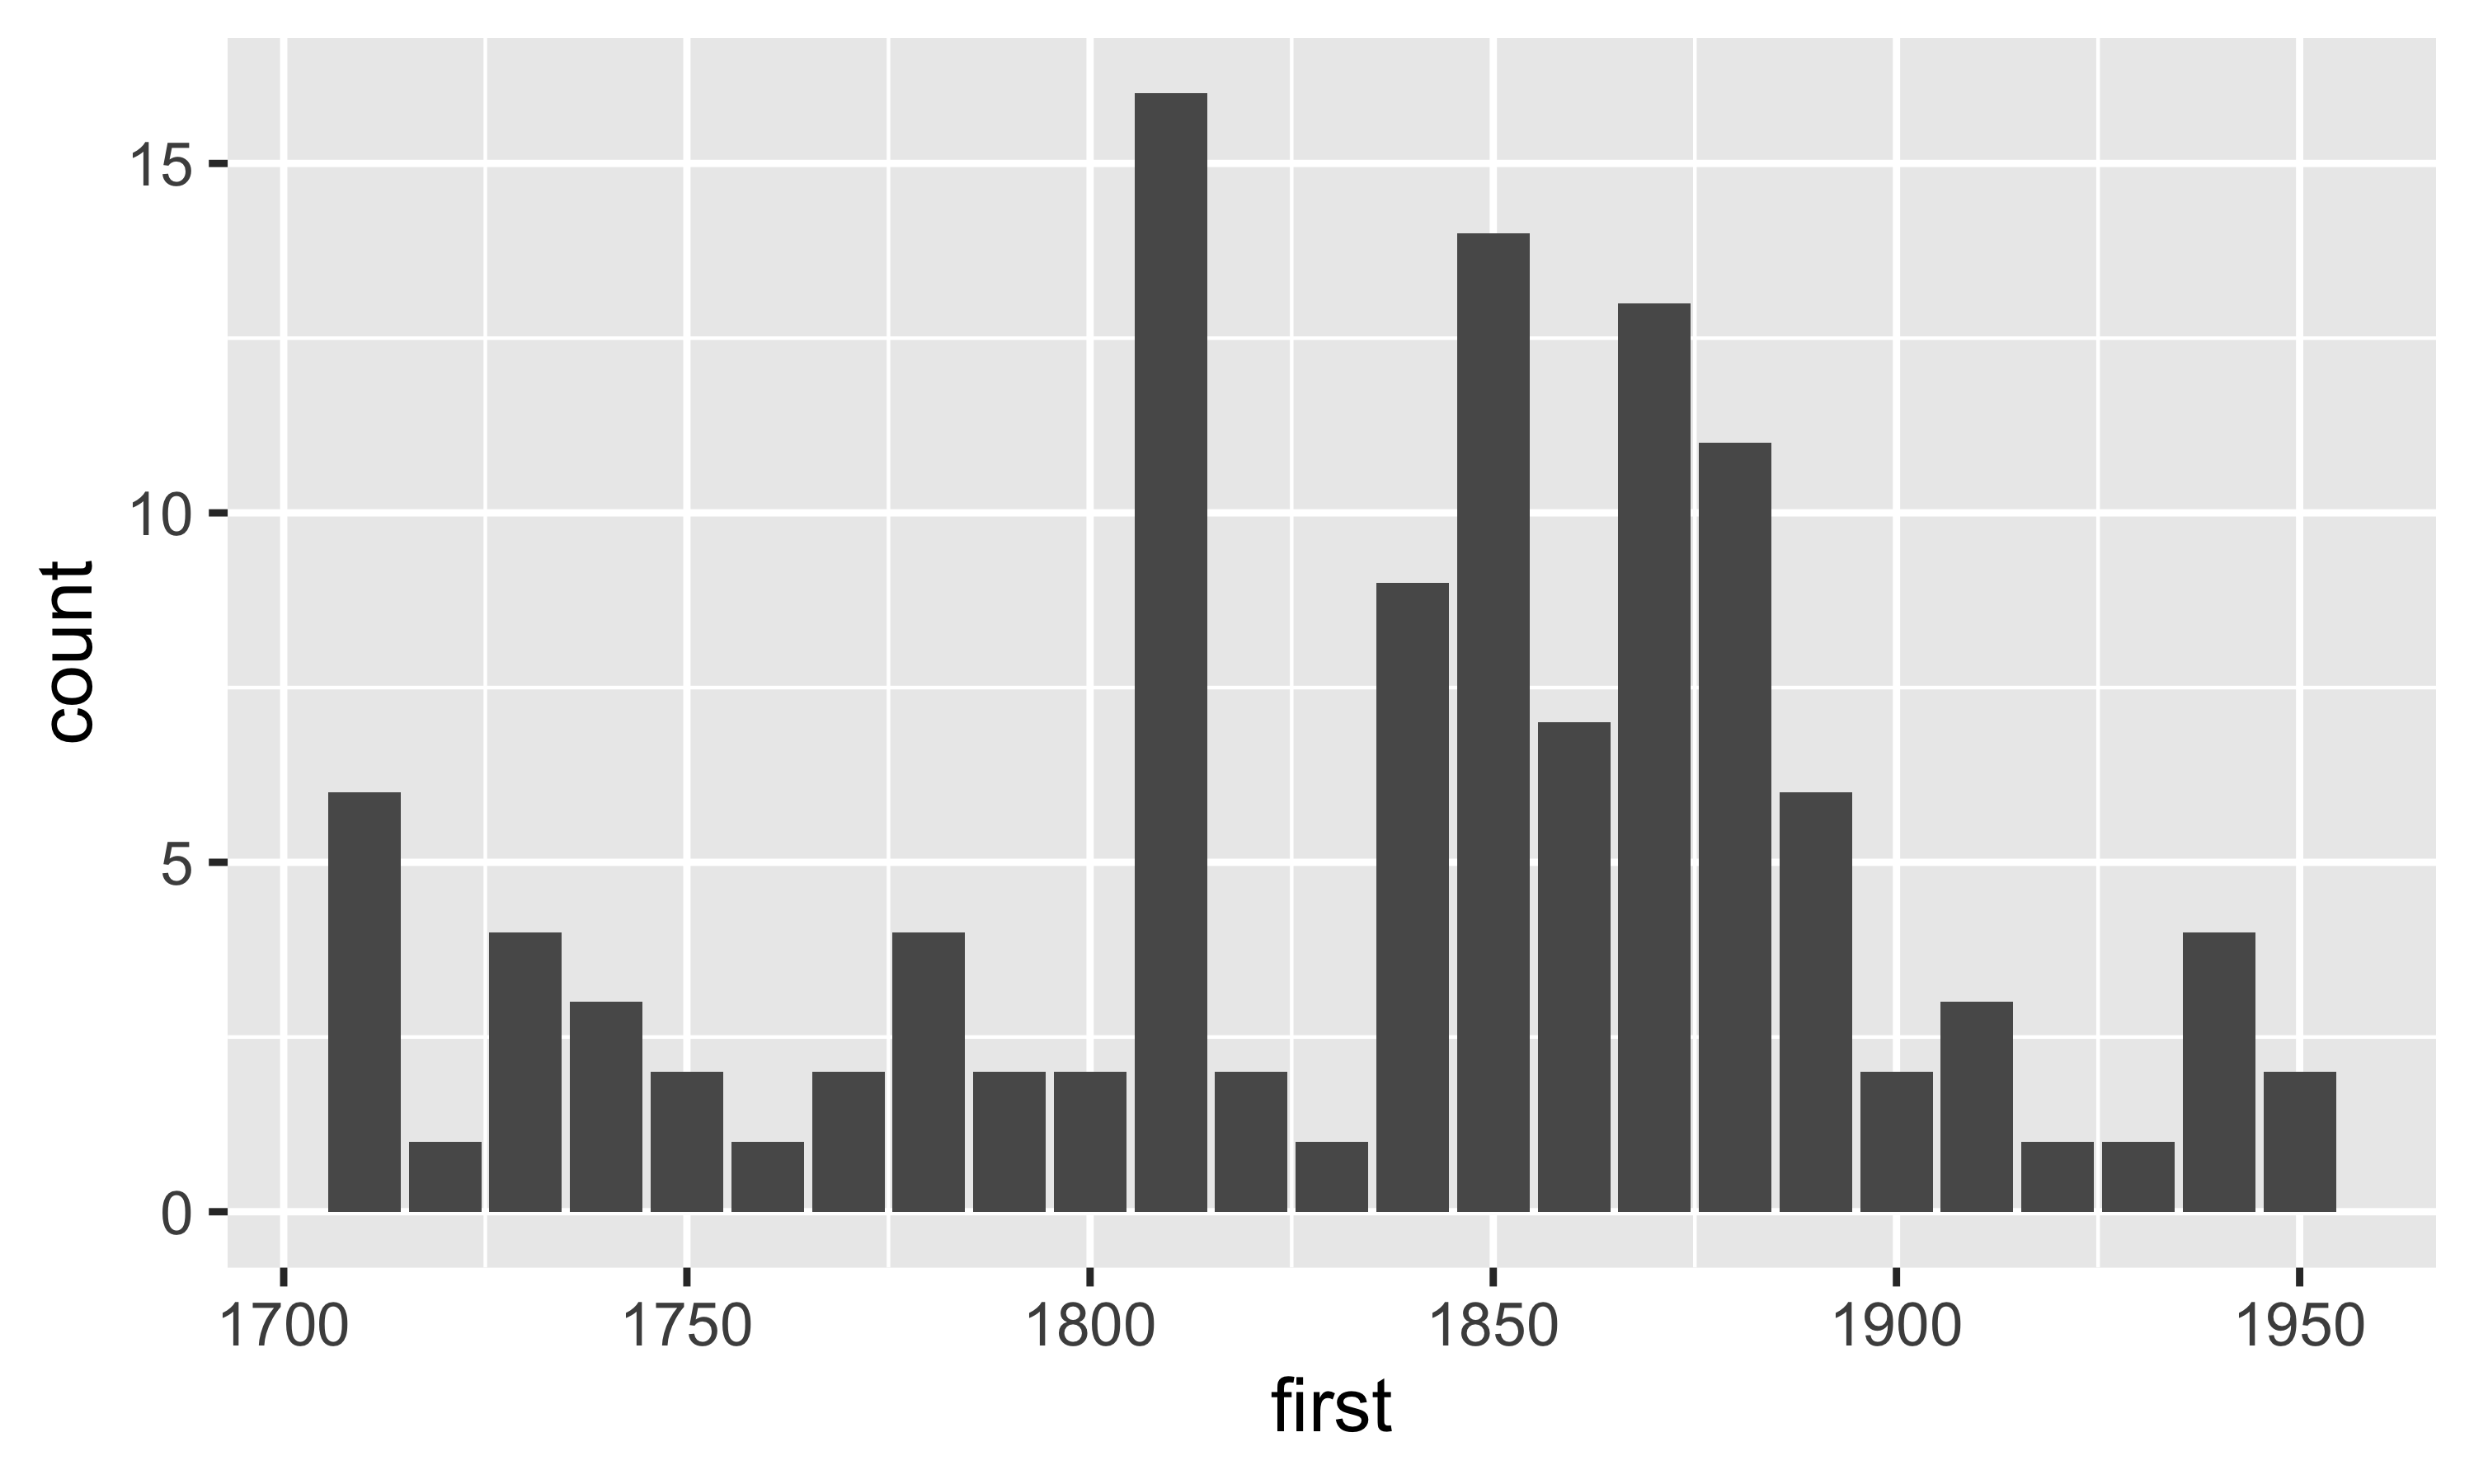
\includegraphics[width=0.6\linewidth]{brolgar-paper_files/figure-latex/feature-first-gg-1} 

}

\caption{Distribution of starting years of measurement. The data is already binned into 10 year blocks. Most of the years start between 1840 and 1900.}\label{fig:feature-first-gg}
\end{figure}

We can explore the variation in first year using \texttt{feat\_diff\_summary}. This combines many summaries of the differences in \texttt{year}.

\begin{verbatim}
heights_diffs <- heights_brolgar %>% 
  features(year, feat_diff_summary)

heights_diffs
\end{verbatim}

\begin{verbatim}
#> # A tibble: 119 x 10
#>    country     diff_min diff_q25 diff_~1 diff_~2 diff_~3 diff_~4 diff_~5 diff_sd
#>    <chr>          <dbl>    <dbl>   <dbl>   <dbl>   <dbl>   <dbl>   <dbl>   <dbl>
#>  1 Afghanistan       10       10      30    32.5    55.8      60   692.    26.3 
#>  2 Algeria           10       10      10    22.5    39.2      60   625     25   
#>  3 Angola            10       10      10    17.5    10        70   450     21.2 
#>  4 Argentina         10       10      10    11.6    10        40    47.4    6.88
#>  5 Armenia           10       10      10    15      20.8      30    72.2    8.50
#>  6 Australia         10       10      10    13.3    10        40   100     10   
#>  7 Austria           10       10      10    13.5    10        40    74.3    8.62
#>  8 Azerbaijan        10       10      10    25      25.8      90  1030     32.1 
#>  9 Bangladesh        10       10      10    18.8    15.8      70   441.    21.0 
#> 10 Belgium           10       10      10    16.7    23.3      40   125     11.2 
#> # ... with 109 more rows, 1 more variable: diff_iqr <dbl>, and abbreviated
#> #   variable names 1: diff_median, 2: diff_mean, 3: diff_q75, 4: diff_max,
#> #   5: diff_var
\end{verbatim}

This is particularly useful as using \texttt{diff} on \texttt{year} would return a very wide dataset that is hard to explore:

\begin{verbatim}
heights_brolgar %>% 
  features(year, diff)
\end{verbatim}

\begin{verbatim}
#> # A tibble: 119 x 30
#>    country      ...1  ...2  ...3  ...4  ...5  ...6  ...7  ...8  ...9 ...10 ...11
#>    <chr>       <dbl> <dbl> <dbl> <dbl> <dbl> <dbl> <dbl> <dbl> <dbl> <dbl> <dbl>
#>  1 Afghanistan    10    50    60    10    NA    NA    NA    NA    NA    NA    NA
#>  2 Algeria        10    10    60    10    NA    NA    NA    NA    NA    NA    NA
#>  3 Angola         10    10    70    10    10    10    10    10    NA    NA    NA
#>  4 Argentina      10    10    10    10    10    10    10    10    10    10    10
#>  5 Armenia        10    30    10    10    30    20    10    10    10    10    NA
#>  6 Australia      10    10    10    10    10    10    10    40    10    NA    NA
#>  7 Austria        20    10    10    30    10    10    10    10    10    10    10
#>  8 Azerbaijan     10    90    10    10    10    20    NA    NA    NA    NA    NA
#>  9 Bangladesh     10    10    10    70    10    20    10    10    NA    NA    NA
#> 10 Belgium        10    10    10    10    10    10    30    40    20    NA    NA
#> # ... with 109 more rows, and 18 more variables: ...12 <dbl>, ...13 <dbl>,
#> #   ...14 <dbl>, ...15 <dbl>, ...16 <dbl>, ...17 <dbl>, ...18 <dbl>,
#> #   ...19 <dbl>, ...20 <dbl>, ...21 <dbl>, ...22 <dbl>, ...23 <dbl>,
#> #   ...24 <dbl>, ...25 <dbl>, ...26 <dbl>, ...27 <dbl>, ...28 <dbl>,
#> #   ...29 <dbl>
\end{verbatim}

We can then look at the summaries of the differences in year by changing to long form and facetting (Figure \ref{fig:heights-long-feat-diff}), we learn about the range of intervals between measurements, the smallest being 10 years, the largest being 125, and that most of the data is measured between 10 and 30 years.

\begin{figure}

{\centering 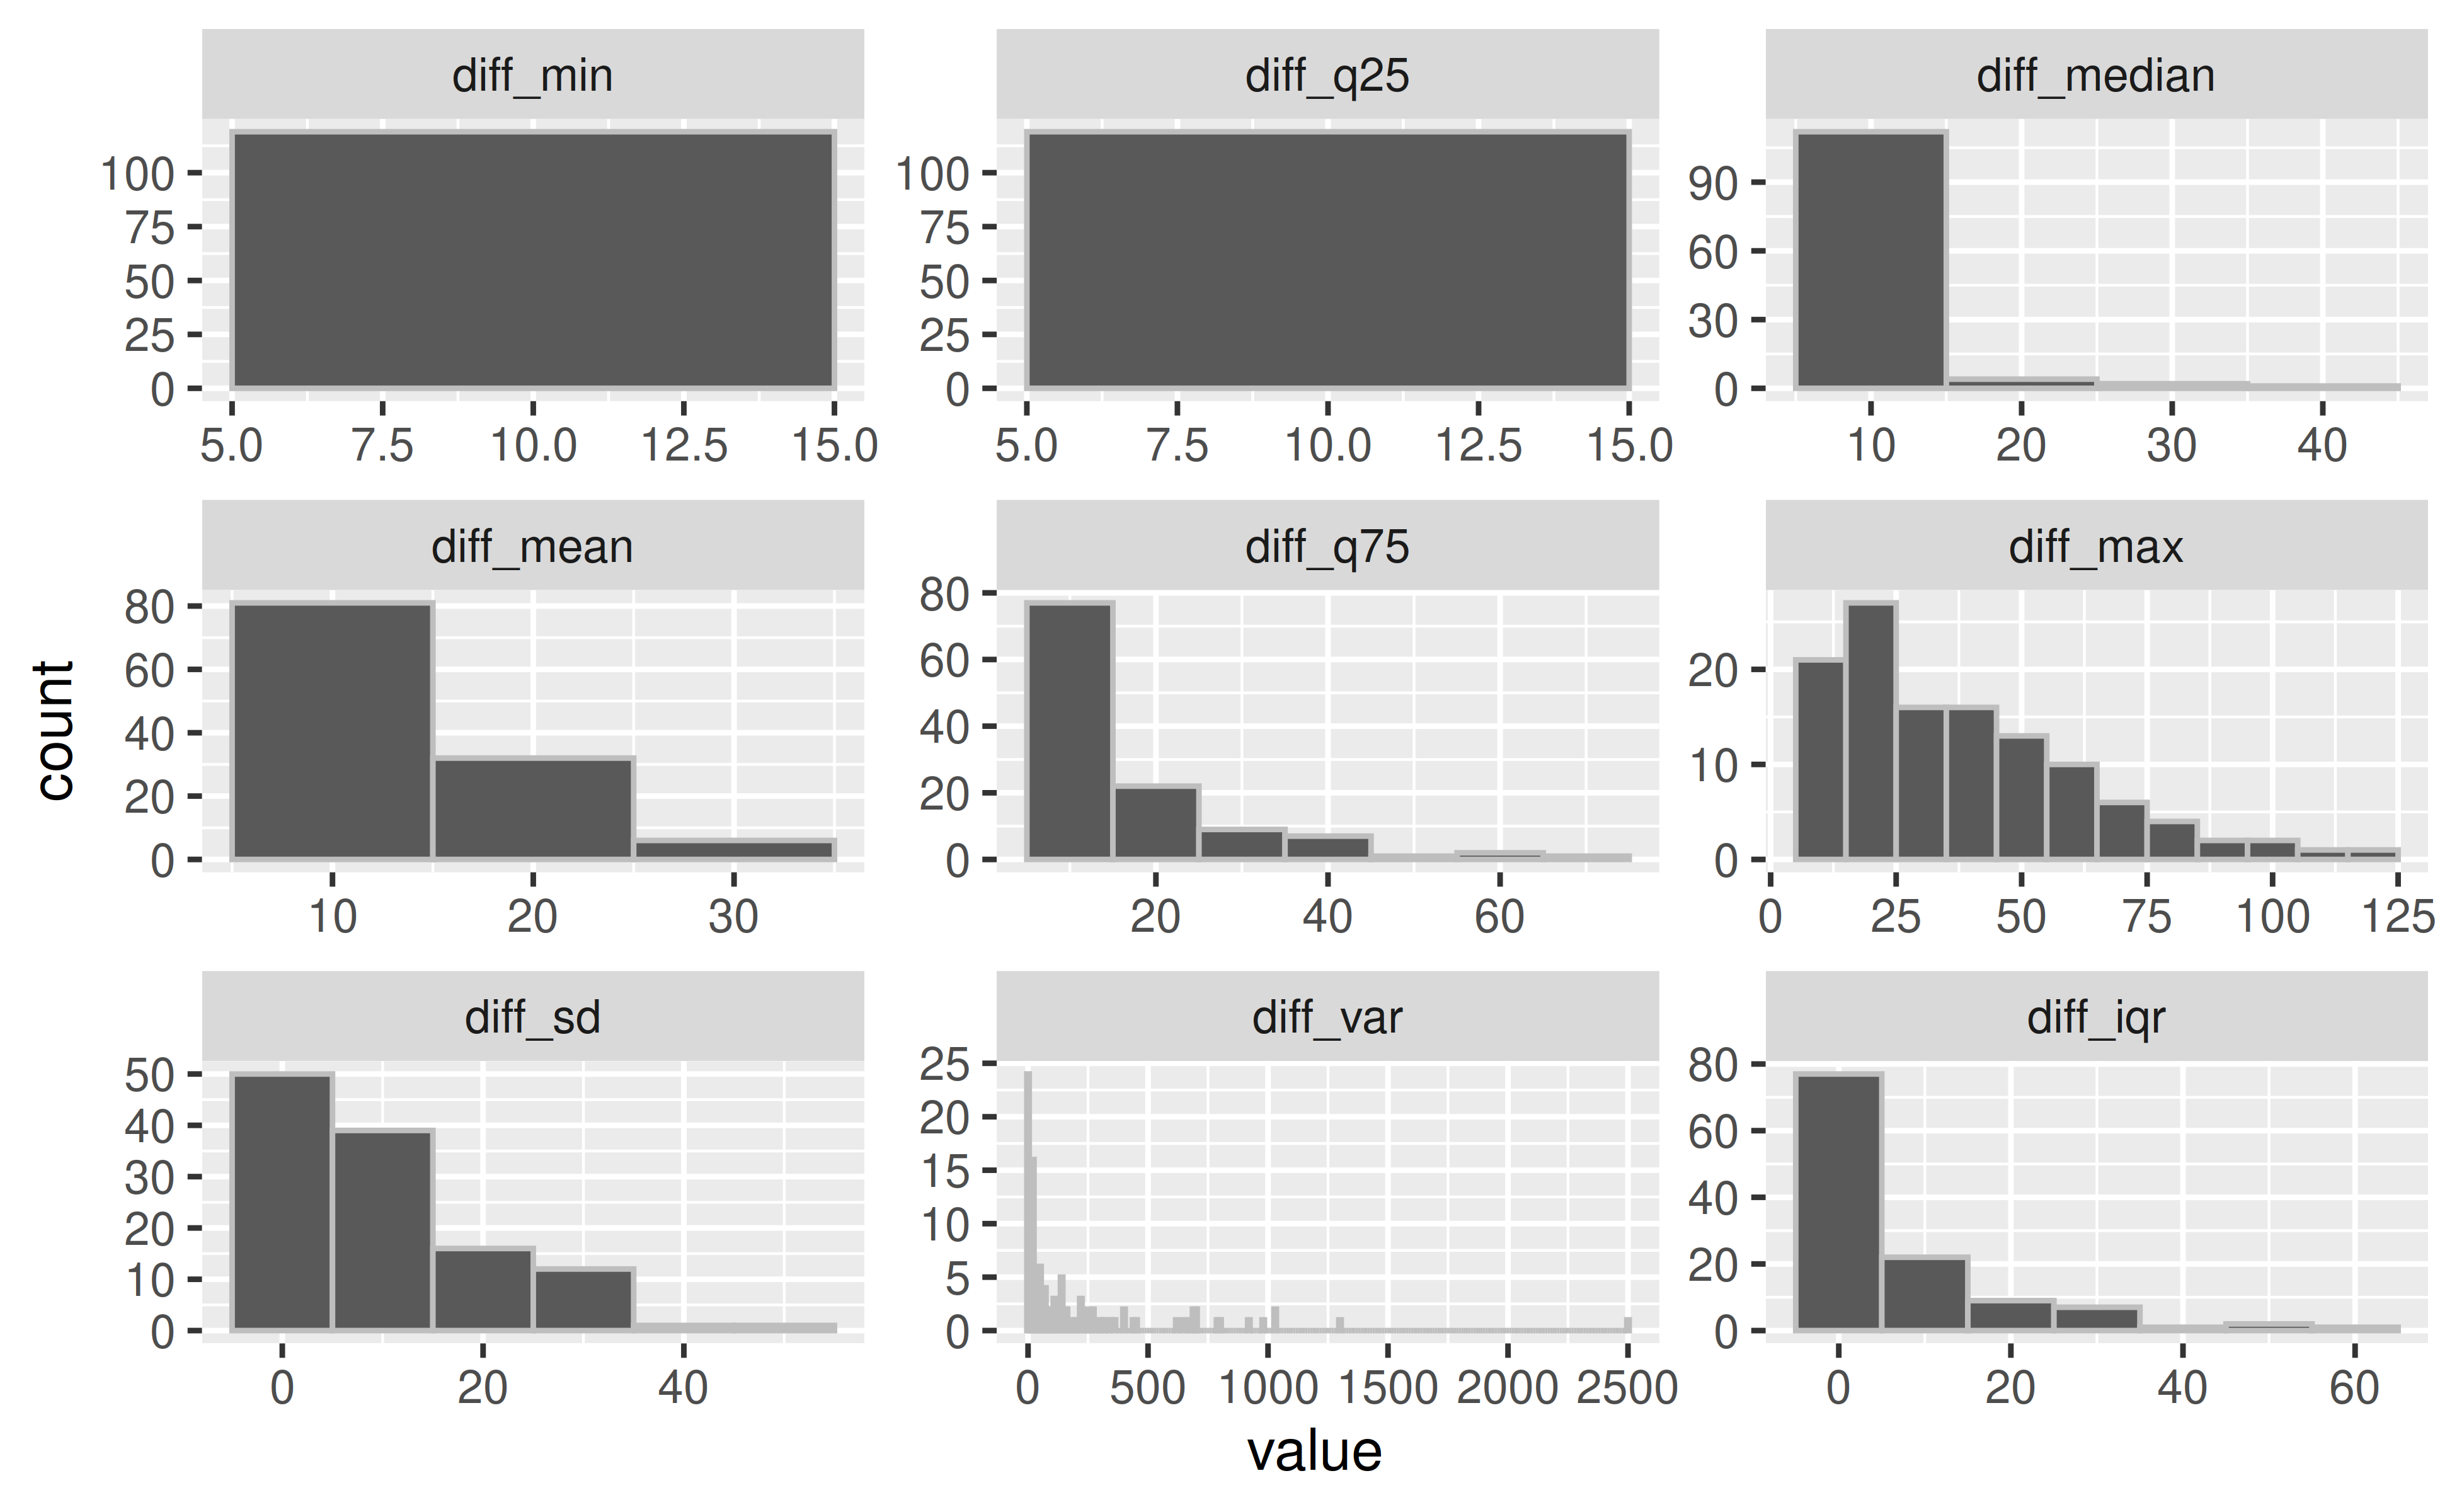
\includegraphics[width=0.95\linewidth]{brolgar-paper_files/figure-latex/heights-long-feat-diff-1} 

}

\caption{Exploring the different summary statistics of the differences amongst the years. We learn that the smallest interval between measurements is 10 years, and the largest interval is between 10 and 125 years, and that most of the data is measured between 10 and 30 or so years.}\label{fig:heights-long-feat-diff}
\end{figure}

\hypertarget{finding-waldo}{%
\section{Finding Waldo}\label{finding-waldo}}

Looking at a spaghetti plot, it can be hard to identify which lines are the most interesting, or unusual. A workflow to identify interesting individuals to start with is given below:

\begin{enumerate}
\def\labelenumi{\arabic{enumi}.}
\tightlist
\item
  Decide upon an interesting feature (e.g., maximum)
\item
  This feature produces one value per key
\item
  Examine the distribution of the feature
\item
  Join this table back to the data to get all observations for those keys
\item
  Arrange the keys or filter, using the feature
\item
  Display the data for selected keys
\end{enumerate}

This workflow is now demonstrated. Firstly, we \textbf{decide on an interesting feature}, ``maximum height'', and whether height is always increasing. We calculate our own ``feature'', calculating maximum height, and whether a value is increasing (with brolgar's \texttt{increasing} function) as follows:

\begin{verbatim}
heights_max_in <- heights_brolgar %>% 
  features(height_cm, list(max = max,
                           increase = increasing))

heights_max_in
\end{verbatim}

\begin{verbatim}
#> # A tibble: 119 x 3
#>    country       max increase
#>    <chr>       <dbl> <lgl>   
#>  1 Afghanistan  168. FALSE   
#>  2 Algeria      171. FALSE   
#>  3 Angola       169. FALSE   
#>  4 Argentina    174. FALSE   
#>  5 Armenia      172. FALSE   
#>  6 Australia    178. FALSE   
#>  7 Austria      179. FALSE   
#>  8 Azerbaijan   172. FALSE   
#>  9 Bangladesh   164. FALSE   
#> 10 Belgium      177. FALSE   
#> # ... with 109 more rows
\end{verbatim}

This returns a dataset of \textbf{one value per key}. Figure \ref{fig:heights-max-in-examine} \textbf{examines the distribution of the features}, showing us the distribution of maximum height, and the number of countries that are always increasing.

\begin{figure}

{\centering 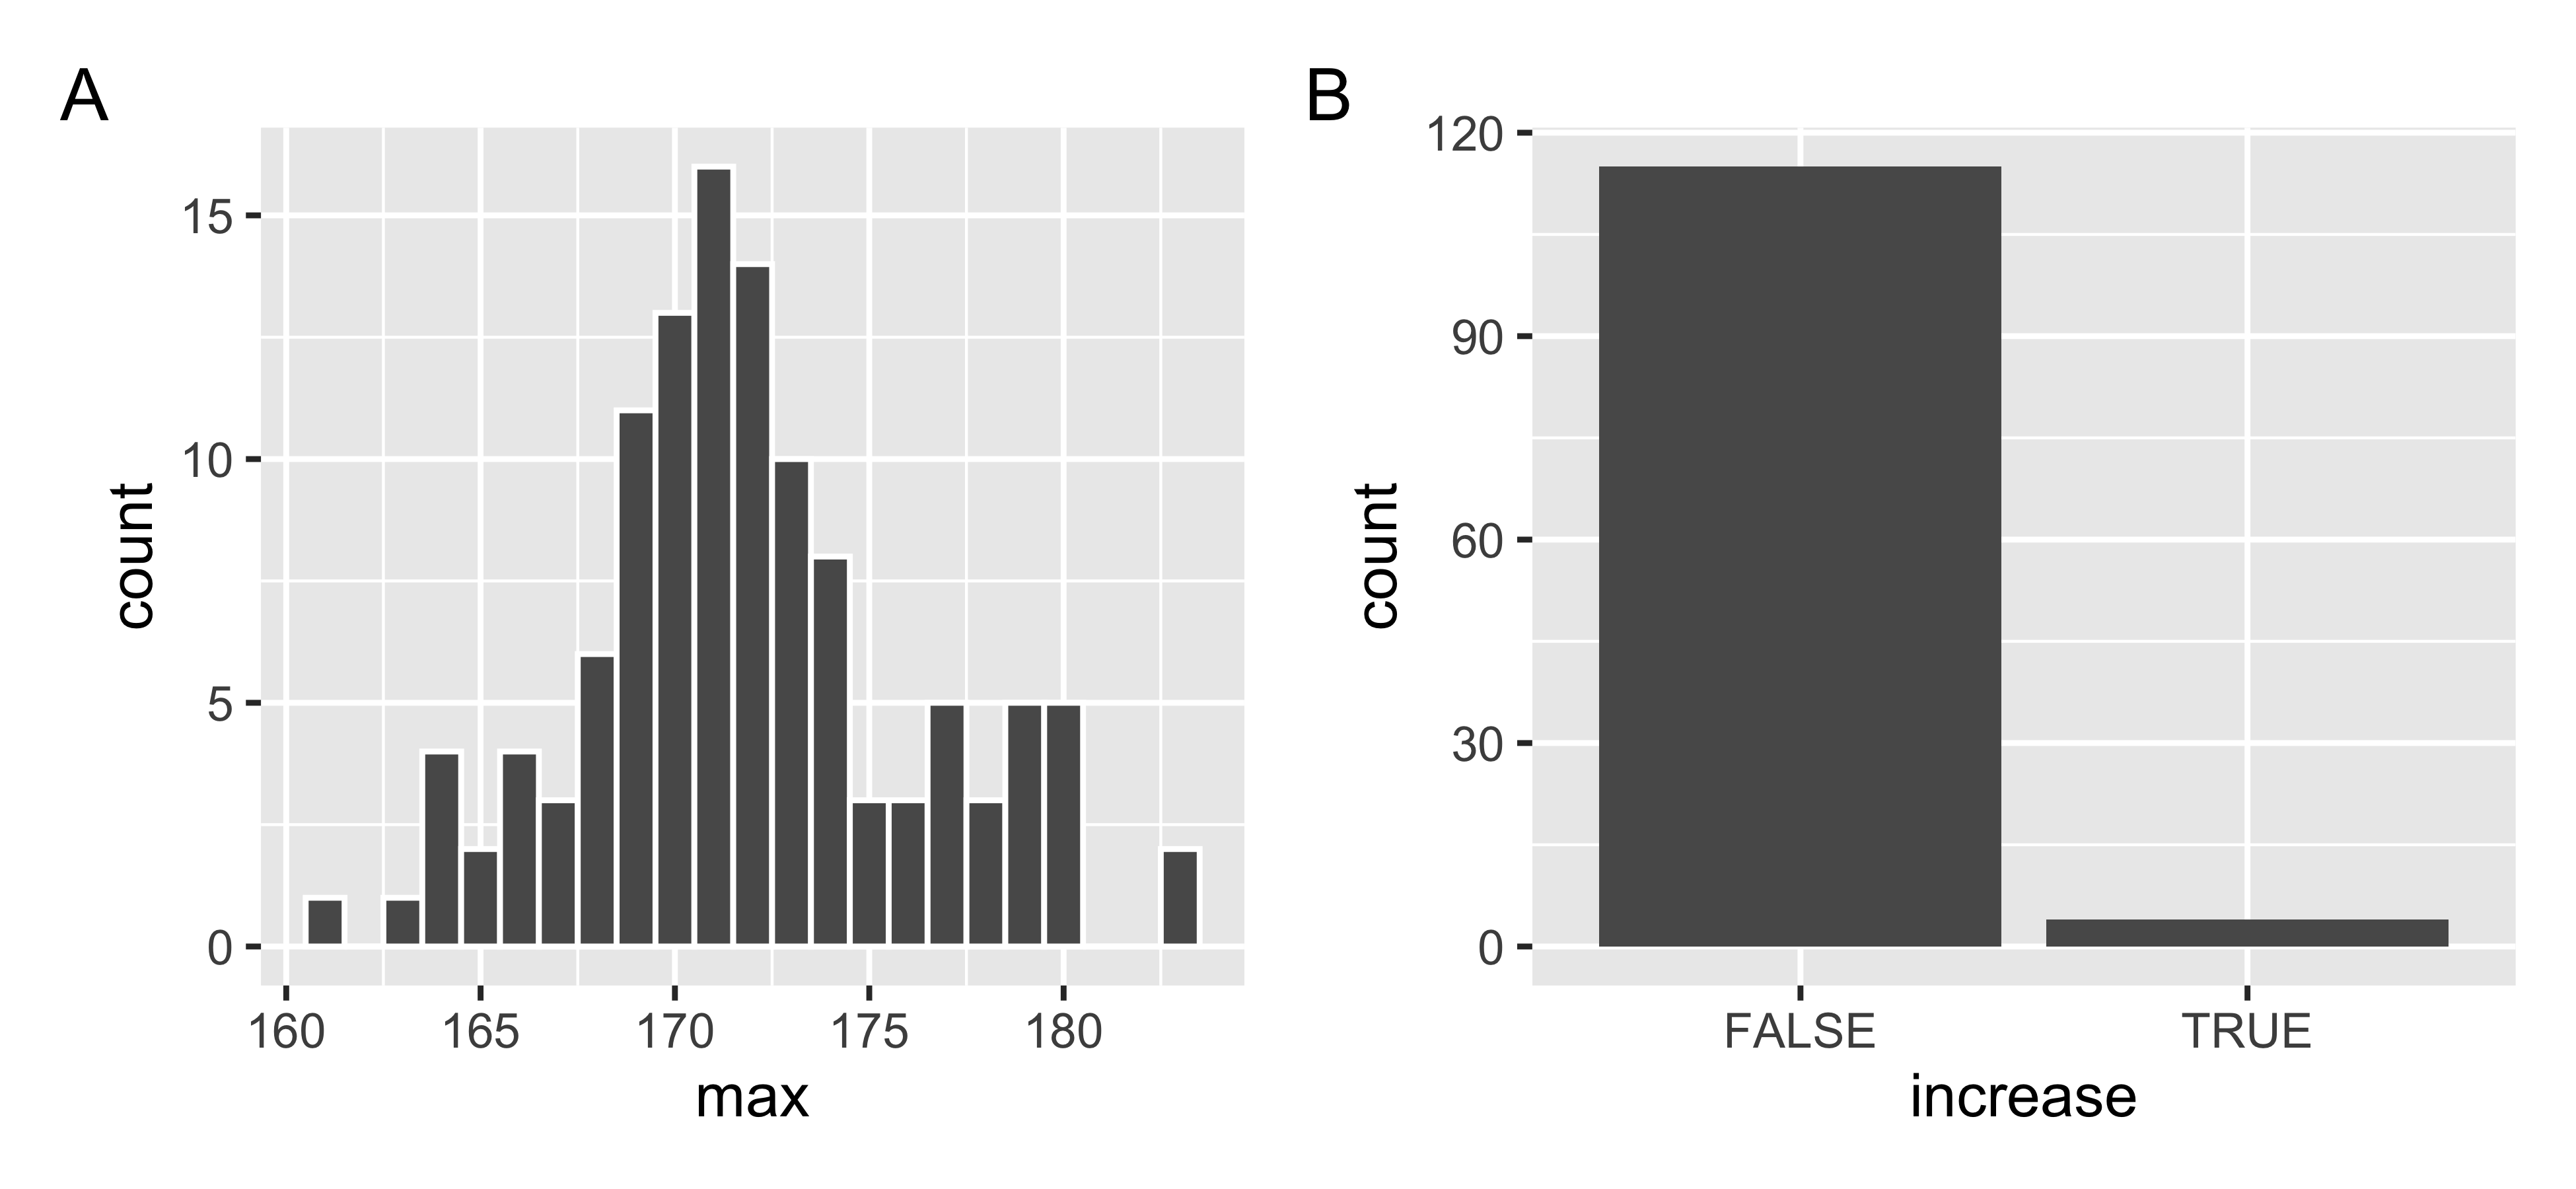
\includegraphics[width=0.95\linewidth]{brolgar-paper_files/figure-latex/heights-max-in-examine-1} 

}

\caption{The different distributions of the features - A is depicting the distribution of maximum height, and B displays the number of countries that are always increasing (FALSE), and always increasing (TRUE). We note that the average maximum heights range from about 160cm to 185cm, with most being around 170cm. We also learn that the vast majority of countries are not always increasing in height through time.}\label{fig:heights-max-in-examine}
\end{figure}

We can now \textbf{join this table back to the data to get all observations for those keys} to move from one key per row to all many rows per key.

\begin{verbatim}
heights_max_in_full <- heights_max_in %>% 
  left_join(heights_brolgar,
            by = "country")

heights_max_in_full
\end{verbatim}

\begin{verbatim}
#> # A tibble: 1,406 x 9
#>    country       max increase  year n_obs continent height_cm year0 country_fct
#>    <chr>       <dbl> <lgl>    <dbl> <int> <chr>         <dbl> <dbl> <fct>      
#>  1 Afghanistan  168. FALSE     1870     5 Asia           168.   160 Afghanistan
#>  2 Afghanistan  168. FALSE     1880     5 Asia           166.   170 Afghanistan
#>  3 Afghanistan  168. FALSE     1930     5 Asia           167.   220 Afghanistan
#>  4 Afghanistan  168. FALSE     1990     5 Asia           167.   280 Afghanistan
#>  5 Afghanistan  168. FALSE     2000     5 Asia           161.   290 Afghanistan
#>  6 Algeria      171. FALSE     1910     5 Africa         169.   200 Algeria    
#>  7 Algeria      171. FALSE     1920     5 Africa         166.   210 Algeria    
#>  8 Algeria      171. FALSE     1930     5 Africa         169    220 Algeria    
#>  9 Algeria      171. FALSE     1990     5 Africa         171.   280 Algeria    
#> 10 Algeria      171. FALSE     2000     5 Africa         170.   290 Algeria    
#> # ... with 1,396 more rows
\end{verbatim}

We can then \textbf{arrange the keys or filter, using the feature}, for example, filtering only those countries that are only increasing:

\begin{verbatim}
heights_increase <- heights_max_in_full %>% filter(increase)
heights_increase
\end{verbatim}

\begin{verbatim}
#> # A tibble: 22 x 9
#>    country    max increase  year n_obs continent height_cm year0 country_fct
#>    <chr>    <dbl> <lgl>    <dbl> <int> <chr>         <dbl> <dbl> <fct>      
#>  1 Honduras  168. TRUE      1950     6 Americas       164.   240 Honduras   
#>  2 Honduras  168. TRUE      1960     6 Americas       164.   250 Honduras   
#>  3 Honduras  168. TRUE      1970     6 Americas       165.   260 Honduras   
#>  4 Honduras  168. TRUE      1980     6 Americas       165.   270 Honduras   
#>  5 Honduras  168. TRUE      1990     6 Americas       165.   280 Honduras   
#>  6 Honduras  168. TRUE      2000     6 Americas       168.   290 Honduras   
#>  7 Moldova   174. TRUE      1840     5 Europe         165.   130 Moldova    
#>  8 Moldova   174. TRUE      1950     5 Europe         172.   240 Moldova    
#>  9 Moldova   174. TRUE      1960     5 Europe         173.   250 Moldova    
#> 10 Moldova   174. TRUE      1970     5 Europe         174.   260 Moldova    
#> # ... with 12 more rows
\end{verbatim}

Or tallest country

\begin{verbatim}
heights_top <- heights_max_in_full %>% top_n(n = 1, wt = max)
heights_top
\end{verbatim}

\begin{verbatim}
#> # A tibble: 16 x 9
#>    country   max increase  year n_obs continent height_cm year0 country_fct
#>    <chr>   <dbl> <lgl>    <dbl> <int> <chr>         <dbl> <dbl> <fct>      
#>  1 Denmark  183. FALSE     1820    16 Europe         167.   110 Denmark    
#>  2 Denmark  183. FALSE     1830    16 Europe         165.   120 Denmark    
#>  3 Denmark  183. FALSE     1850    16 Europe         167.   140 Denmark    
#>  4 Denmark  183. FALSE     1860    16 Europe         168.   150 Denmark    
#>  5 Denmark  183. FALSE     1870    16 Europe         168.   160 Denmark    
#>  6 Denmark  183. FALSE     1880    16 Europe         170.   170 Denmark    
#>  7 Denmark  183. FALSE     1890    16 Europe         169.   180 Denmark    
#>  8 Denmark  183. FALSE     1900    16 Europe         170.   190 Denmark    
#>  9 Denmark  183. FALSE     1910    16 Europe         170    200 Denmark    
#> 10 Denmark  183. FALSE     1920    16 Europe         174.   210 Denmark    
#> 11 Denmark  183. FALSE     1930    16 Europe         174.   220 Denmark    
#> 12 Denmark  183. FALSE     1940    16 Europe         176.   230 Denmark    
#> 13 Denmark  183. FALSE     1950    16 Europe         180.   240 Denmark    
#> 14 Denmark  183. FALSE     1960    16 Europe         180.   250 Denmark    
#> 15 Denmark  183. FALSE     1970    16 Europe         181.   260 Denmark    
#> 16 Denmark  183. FALSE     1980    16 Europe         183.   270 Denmark
\end{verbatim}

We can then display the data by highlighting it in the background, first creating a background plot and overlaying the plots on top of this as an additional ggplot layer, in Figure
\ref{fig:gg-increase-max}.

\begin{figure}

{\centering \includegraphics[width=0.95\linewidth]{brolgar-paper_files/figure-latex/gg-increase-max-1} 

}

\caption{Plots of the data in the background, with the countries that always increase in height through time in A, and the country with the tallest people in B}\label{fig:gg-increase-max}
\end{figure}

\hypertarget{dancing-with-models}{%
\section{Dancing with Models}\label{dancing-with-models}}

These same workflows can be used to interpret and explore a model. As the data tends to follow a non linear trajectory, we use a general additive model (gam) with the \CRANpkg{mgcv} R package (Wood 2017) using the code below:

\begin{verbatim}
heights_gam <- gam(
    height_cm ~ s(year0, by = country_fct) + country_fct,
    data = heights_brolgar,
    method = "REML"
  )
\end{verbatim}

This fits height in centimetres with a smooth effect for year for each country, with a different intercept for each country. It is roughly equivalent to a random intercept varying slope model. Note that this gam model took approximately 8074 seconds to fit. We add the predicted and residual values for the model below, as well as the residual sums of squares for each country.

\begin{verbatim}
library(mgcv)
library(modelr)
heights_aug <- heights_brolgar %>%
  add_predictions(heights_gam, var = "pred") %>%
  add_residuals(heights_gam, var = "res") %>% 
  group_by_key() %>% 
  mutate(rss = sum(res^2)) %>% 
  ungroup()
\end{verbatim}

We can use the previous approach to explore the model results. We can take a look at a sample of the predictions along with the data, by using \texttt{sample\_n\_keys}. This provides a useful way to explore some set of the model predictions. In order to find those predictions that best summarise the best, and worst, and in between, we need to use the methods in the next section, ``Stereotyping''.

\begin{verbatim}
heights_aug %>% 
  sample_n_keys(12) %>% 
  ggplot(aes(x = year,
             y = pred,
             group = country)) + 
  geom_line(colour = "steelblue") +
  geom_point(aes(y = height_cm)) + 
  facet_wrap(~country)
\end{verbatim}

\begin{figure}

{\centering 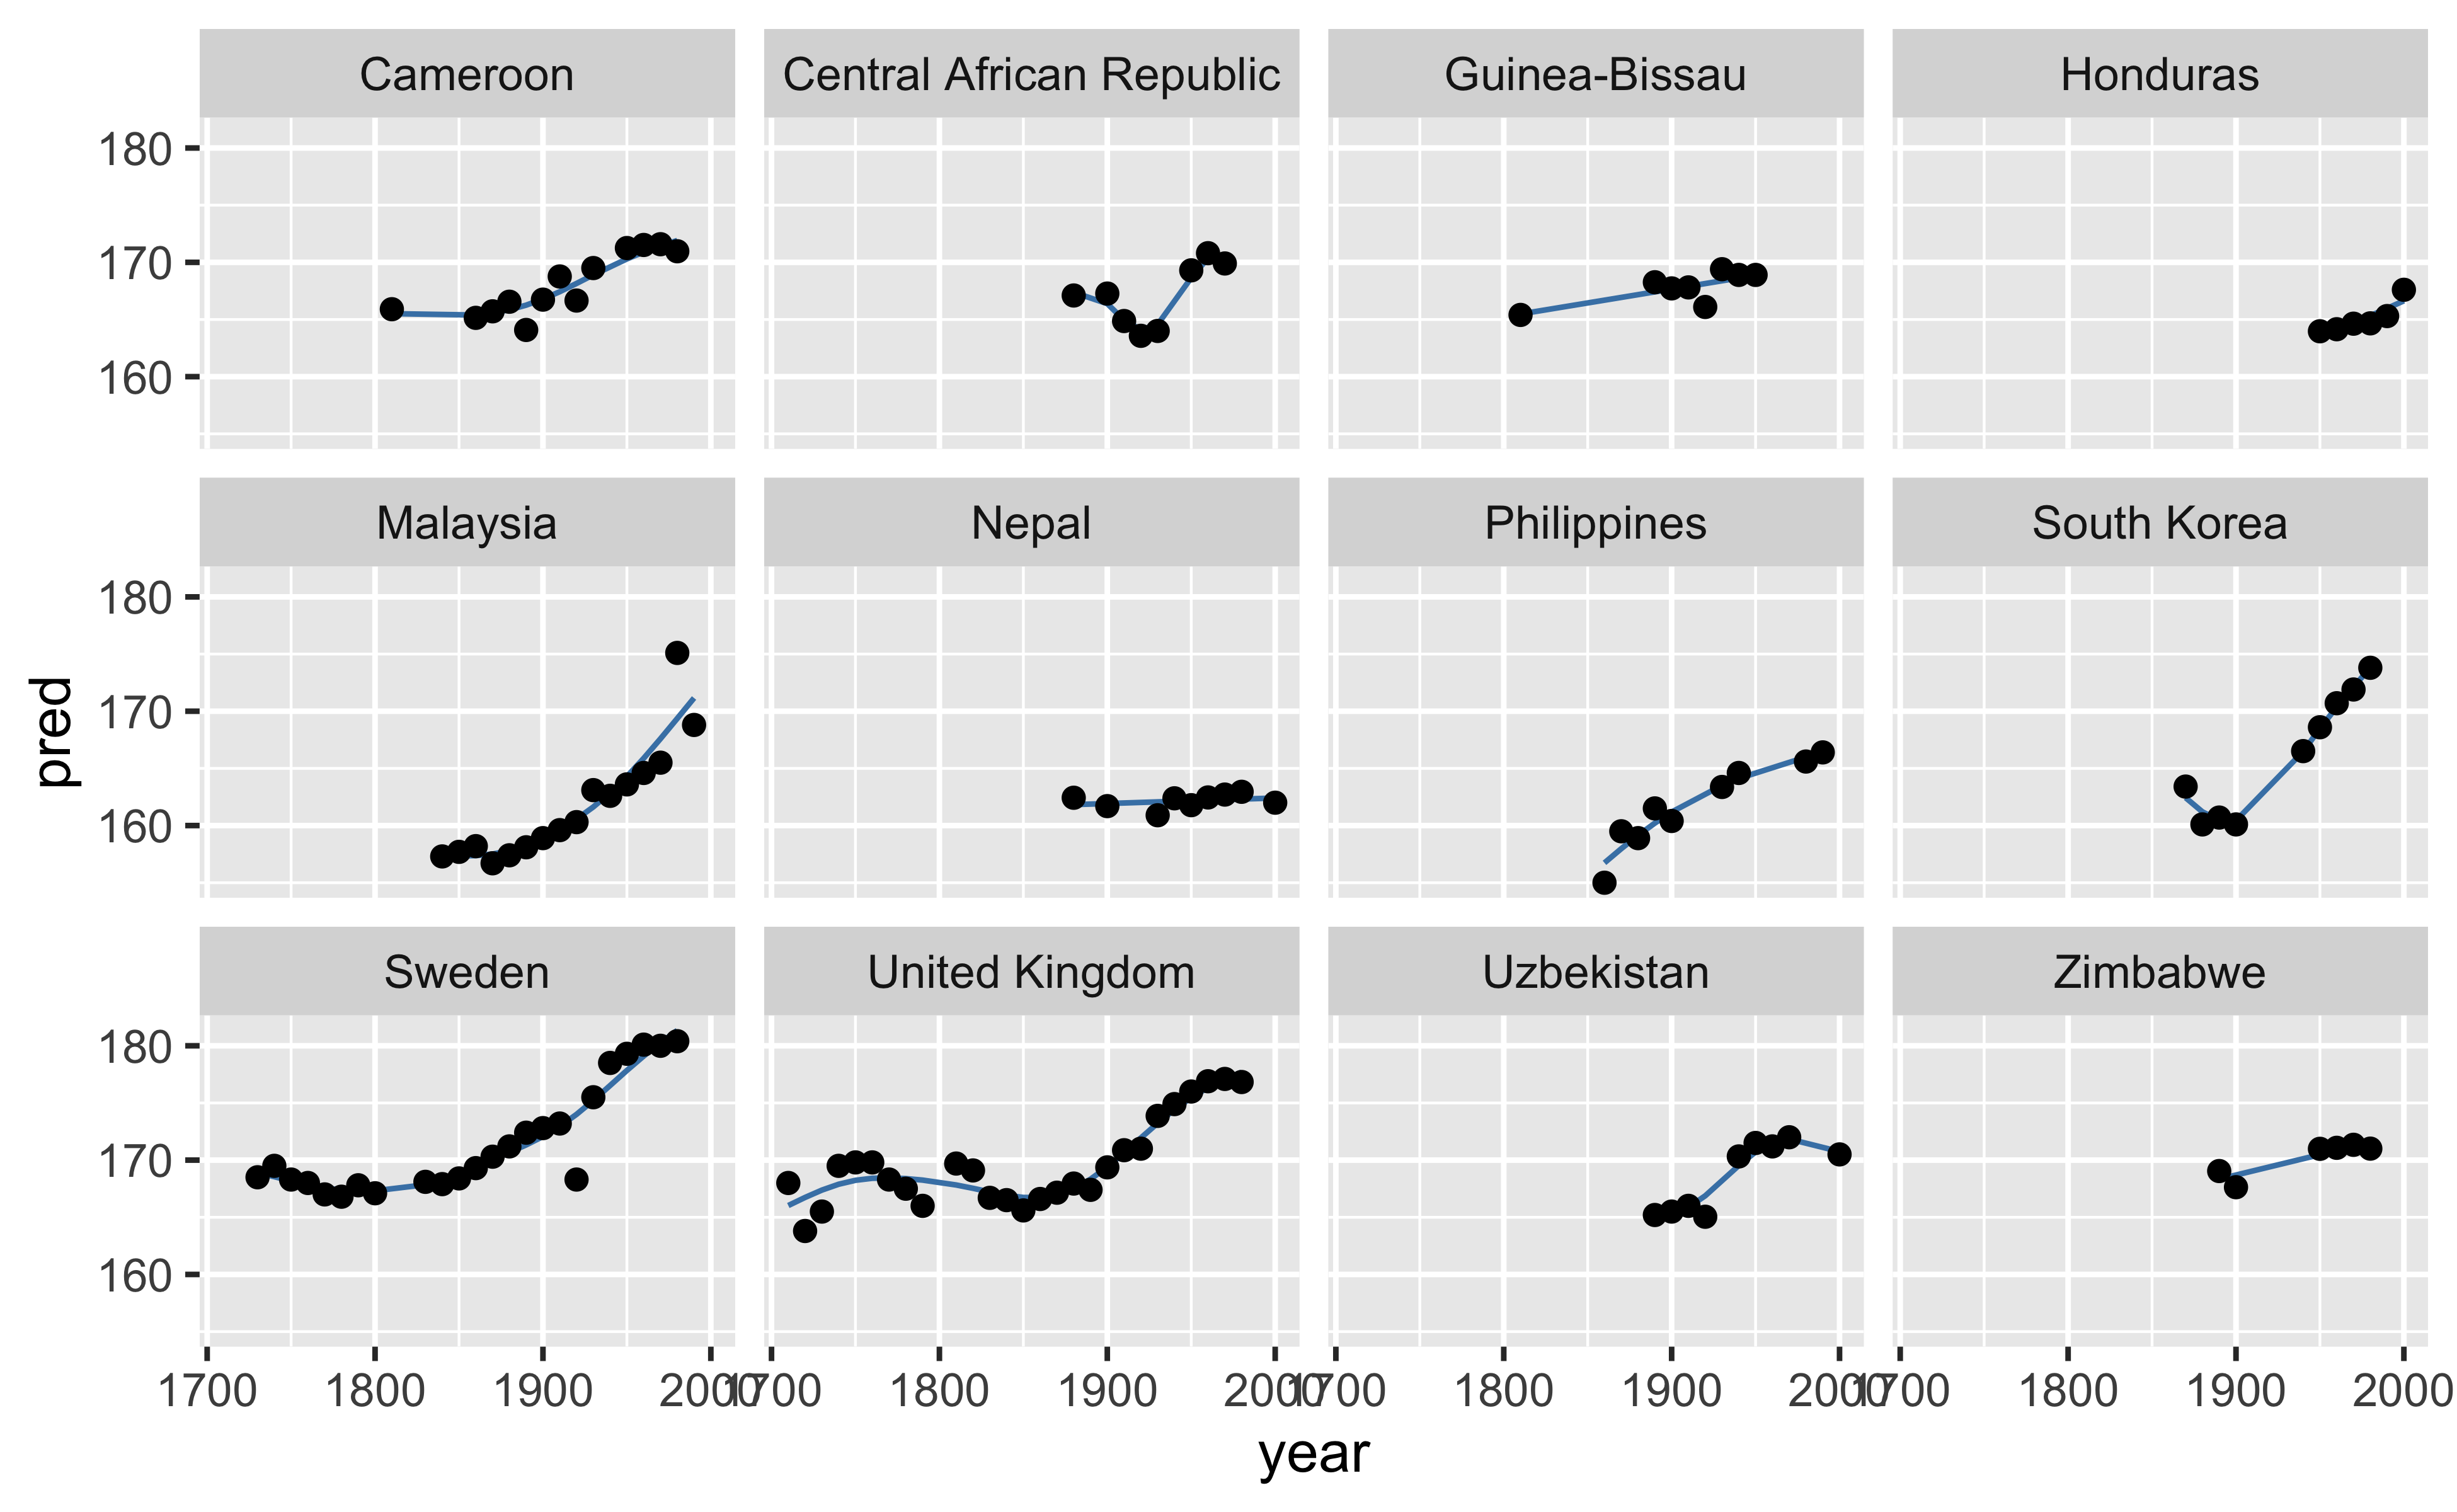
\includegraphics[width=0.95\linewidth]{brolgar-paper_files/figure-latex/sample-n-keys-model-1} 

}

\caption{Exploration of a random sample of the data. This shows the data points of 12 countries, with the model fit in blue.}\label{fig:sample-n-keys-model}
\end{figure}

\hypertarget{stereotyping}{%
\section{Stereotyping}\label{stereotyping}}

To help understand a population of measurements over time, it can be useful to understand which individual measurements are typical (or ``stereotypical'') of a measurement. For example, to understand which individuals are stereotypical of a statistic such as the minimum, median, and maximum height. This section discusses how to find these stereotypes in the data.

Figure \ref{fig:heights-aug-res-summary} shows the residuals of the simple model fit to the data in the previous section. There is an overlaid five number summary, showing the minimum, 1st quantile, median, 3rd quantile, and maximum residual value residuals, as well as a rug plot to show the data. We can use these residuals to understand the stereotypes of the data - those individuals in the model that best match to this five number summary.

\begin{figure}

{\centering 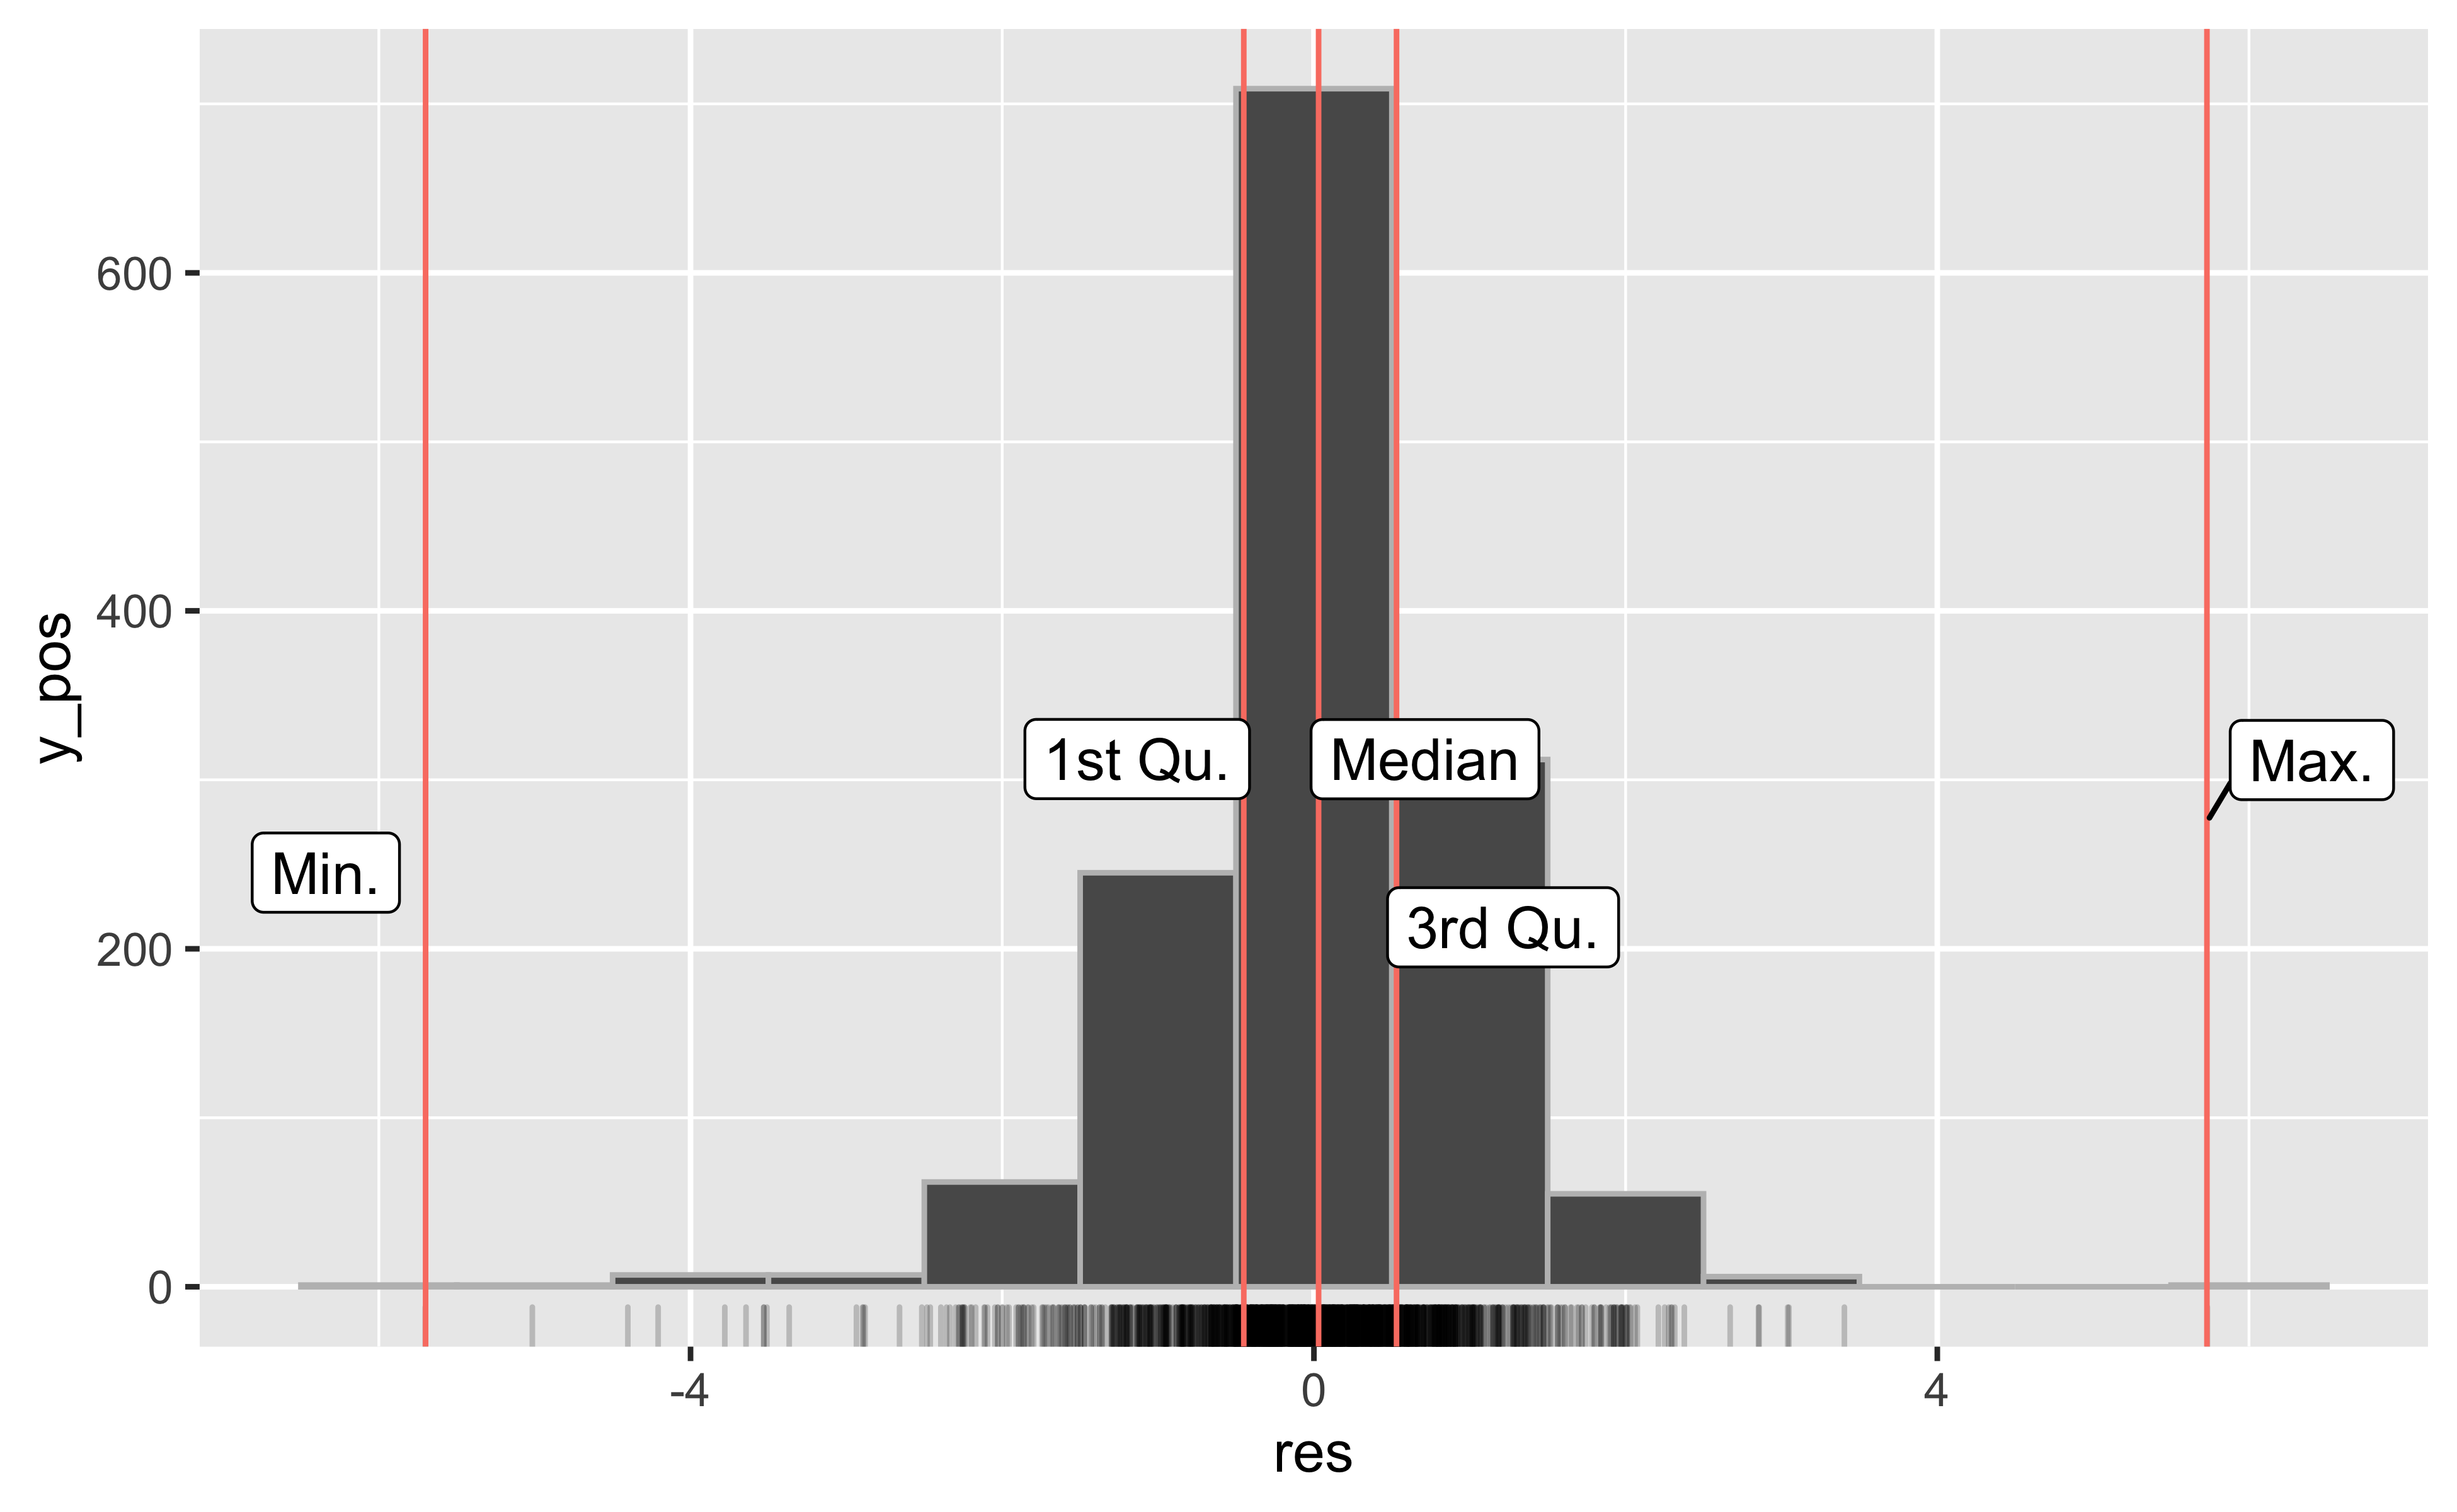
\includegraphics[width=0.6\linewidth]{brolgar-paper_files/figure-latex/heights-aug-res-summary-1} 

}

\caption{Five number summary of residual values from the model fit. The residuals are centered around zero with some variation.}\label{fig:heights-aug-res-summary}
\end{figure}

We can do this using \texttt{keys\_near()} from \texttt{brolgar}. By default this uses the 5 number summary, but any function can be used. You specify the variable you want to find the keys nearest, in this case \texttt{rss}, residual sums of squares for each key:

\begin{verbatim}
keys_near(heights_aug, var = rss)
\end{verbatim}

\begin{verbatim}
#> # A tibble: 62 x 5
#>    country   rss stat  stat_value stat_diff
#>    <chr>   <dbl> <fct>      <dbl>     <dbl>
#>  1 Denmark  9.54 med         9.54         0
#>  2 Denmark  9.54 med         9.54         0
#>  3 Denmark  9.54 med         9.54         0
#>  4 Denmark  9.54 med         9.54         0
#>  5 Denmark  9.54 med         9.54         0
#>  6 Denmark  9.54 med         9.54         0
#>  7 Denmark  9.54 med         9.54         0
#>  8 Denmark  9.54 med         9.54         0
#>  9 Denmark  9.54 med         9.54         0
#> 10 Denmark  9.54 med         9.54         0
#> # ... with 52 more rows
\end{verbatim}

To plot the data, they need to be joined back to the original data, we use a left join, joining by country.

\begin{verbatim}
heights_near_aug <- heights_aug %>% 
  keys_near(var = rss) %>% 
  left_join(heights_aug, 
            by = c("country"))
\end{verbatim}

Figure \ref{fig:heights-keys-near} shows those countries closest to the five number summary. Observing this, we see that the minimum RSS for Moldova fits a nearly perfectly straight line, and the maximum residuals for Myanmar have wide spread of values.

\begin{verbatim}
ggplot(heights_near_aug,
       aes(x = year,
           y = pred,
           group = country,
           colour = country)) + 
  geom_line(colour = "orange") + 
  geom_point(aes(y = height_cm)) + 
  scale_x_continuous(breaks = c(1780, 1880, 1980)) +
  facet_wrap(~stat + country,
             labeller = label_glue("Country: {country} \nNearest to \n{stat} RSS"),
             nrow = 1) + 
  theme(legend.position = "none",
        aspect.ratio = 1)
\end{verbatim}

\begin{figure}

{\centering 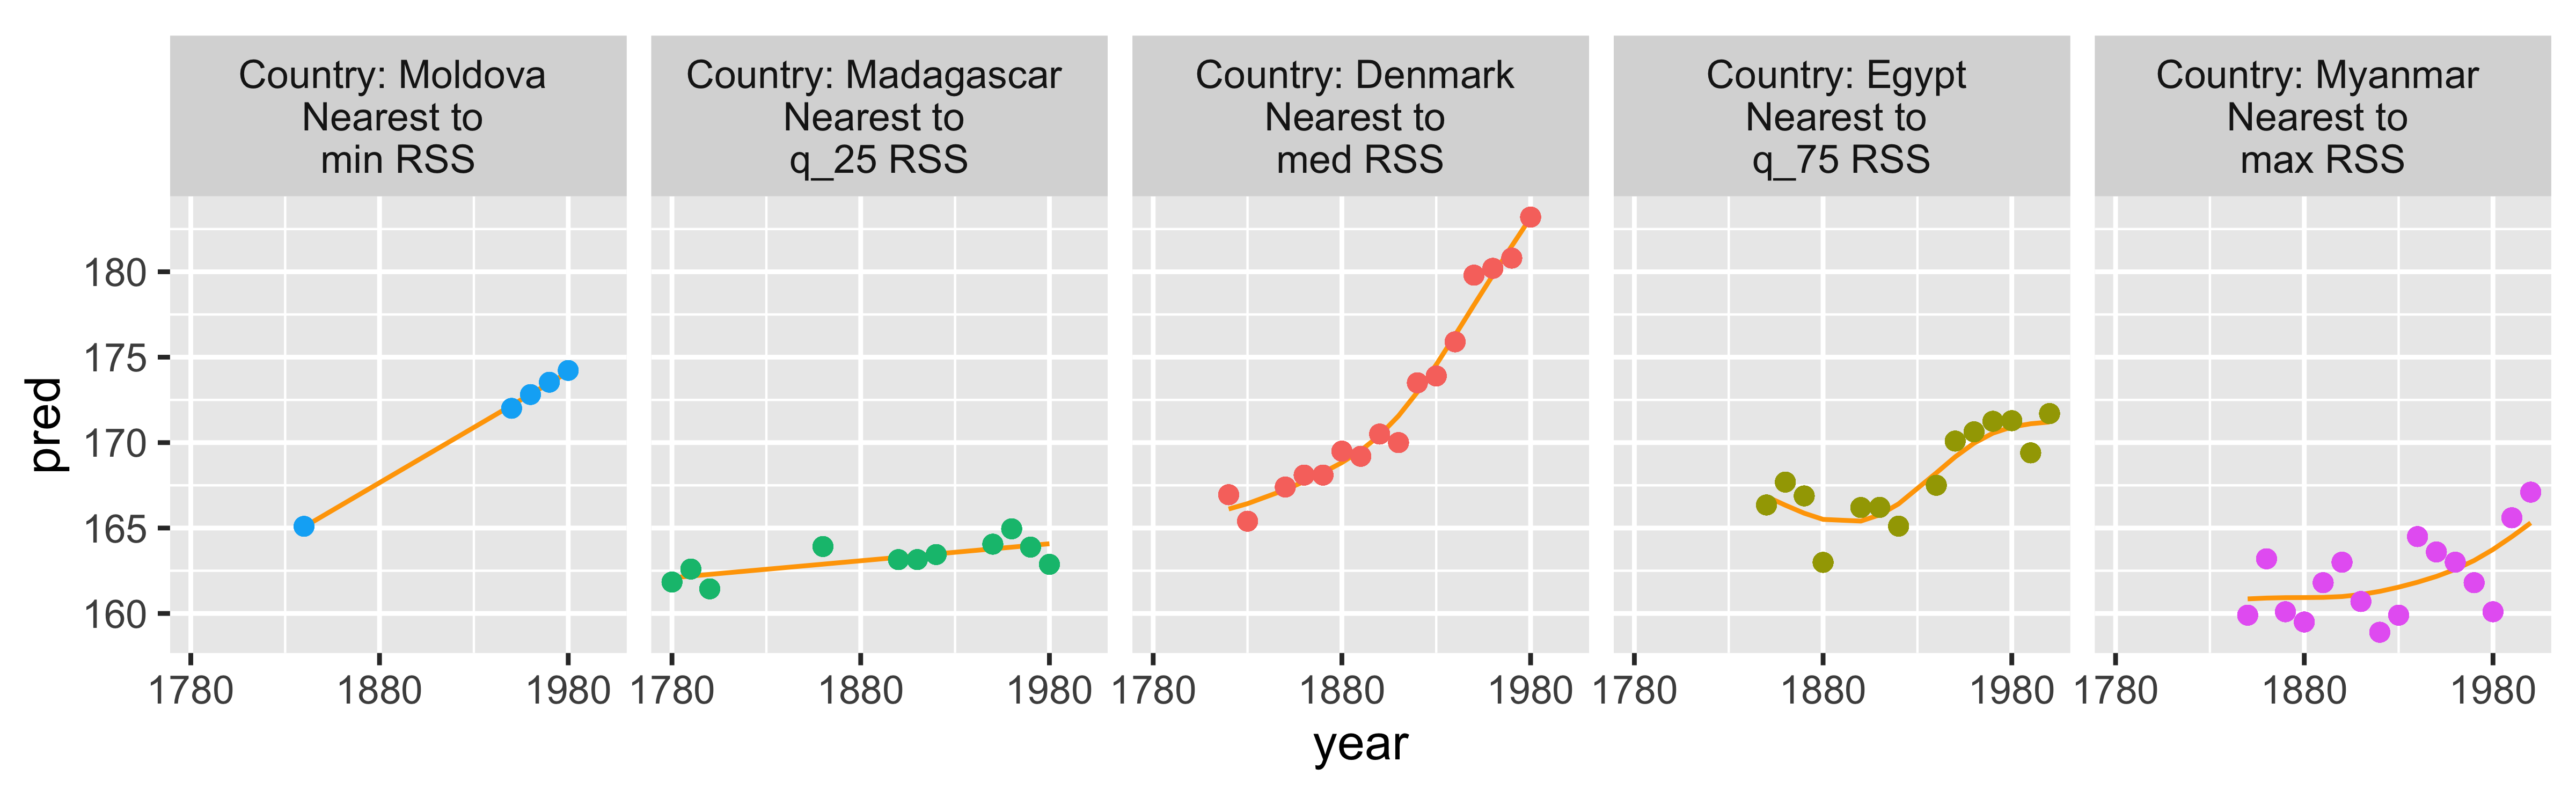
\includegraphics[width=0.95\linewidth]{brolgar-paper_files/figure-latex/heights-keys-near-1} 

}

\caption{The keys nearest to the five number summary of the residual sums of squares. Moldova and Madagascar are well fit by the model, and are fit by a straight line. The remaining countries with poorer fit have greater variation in height. It is not clear how a better model fit could be achieved.}\label{fig:heights-keys-near}
\end{figure}

We can also look at the highest and lowest 3 residual sums of squares:

\begin{verbatim}
heights_near_aug_top_3 <- heights_aug %>% 
  distinct(country, rss) %>% 
  top_n(n = 3,
        wt = rss)

heights_near_aug_bottom_3 <- heights_aug %>% 
  distinct(country, rss) %>% 
  top_n(n = -3,
        wt = rss)

heights_near_top_bot_3 <- bind_rows(highest_3 = heights_near_aug_top_3,
                                    lowest_3 = heights_near_aug_bottom_3,
                                    .id = "rank") %>% 
  left_join(heights_aug,
            by = c("country", "rss"))
\end{verbatim}

Figure \ref{fig:heights-keys-near-fancy-label} shows the same information as the previous plot, but with the 3 representative countries for each statistic. This gives us more data on what the stereotypically ``good'' and ``poor'' fitting countries to this model.

\begin{figure}

{\centering 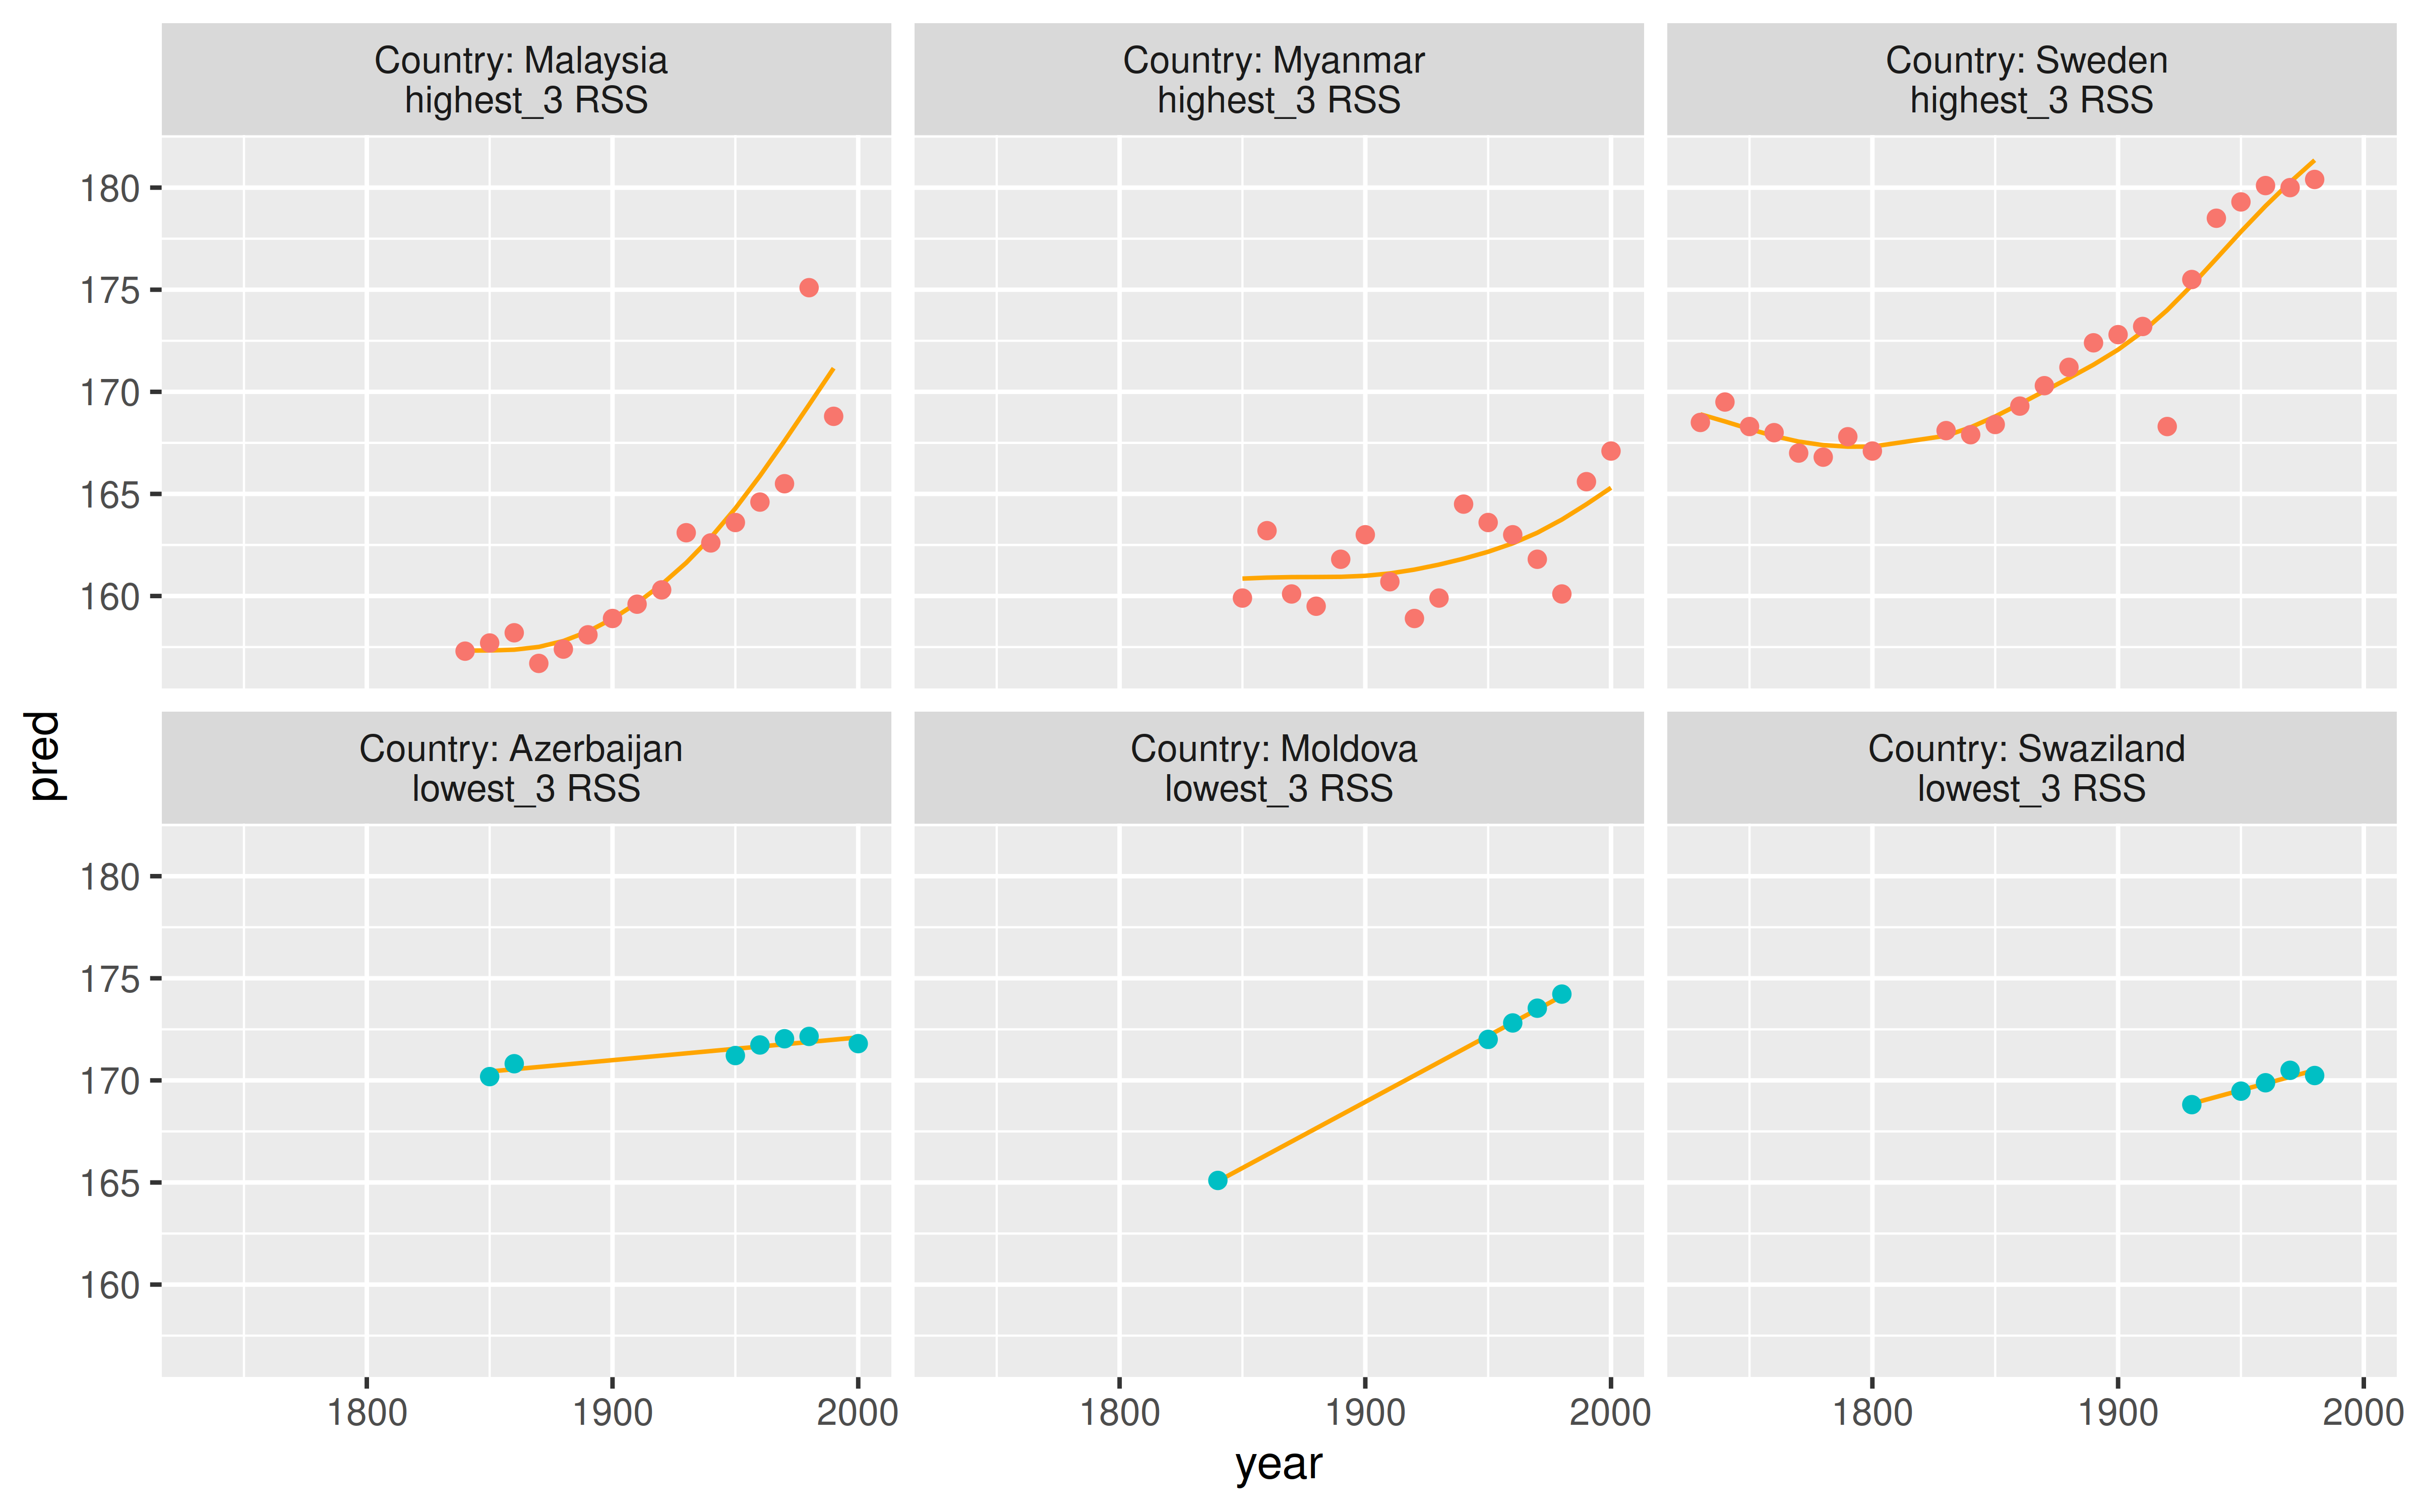
\includegraphics[width=0.95\linewidth]{brolgar-paper_files/figure-latex/heights-keys-near-fancy-label-1} 

}

\caption{Figure of stereotypes for those keys with the three highest and lowest RSS values. Those that fit best tend to be linear, but those that fit worst have wider variation in heights.}\label{fig:heights-keys-near-fancy-label}
\end{figure}

\hypertarget{getting-started}{%
\section{Getting Started}\label{getting-started}}

The \CRANpkg{brolgar} R package can be installed from CRAN using

\begin{verbatim}
# From CRAN
install.packages("brolgar")
# Development version
remotes::install_github("njtierney/brolgar")
\end{verbatim}

The functions are all designed to build upon existing packages, but are predicated on working with \CRANpkg{tsibble}. The package extends upon \CRANpkg{ggplot2} to provide facets for exploration: \texttt{facet\_sample()} and \texttt{facet\_strata()}. Extending \CRANpkg{dplyr}'s \texttt{sample\_n()} and \texttt{sample\_frac()} functions by providing sampling and stratifying based around keys: \texttt{sample\_n\_keys()}, \texttt{sample\_frac\_keys()}, and \texttt{stratify\_keys()}. New functions are focussed around the use of \texttt{key}, for example \texttt{key\_slope()} to find the slope of each key, and \texttt{keys\_near()} to find those keys near a summary statistic. Finally, feature calculation is provided by building upon the existing time series feature package, \CRANpkg{feasts}.

To get started with \CRANpkg{brolgar} you must first ensure your data is specified as a \texttt{tsibble} - discussed earlier in the paper, there is also a vignette \href{http://brolgar.njtierney.com/articles/longitudinal-data-structures.html}{``Longitudinal Data Structures''}, which discusses these ideas. The next step we recommend is sampling some of your data with \texttt{facet\_sample()}, and \texttt{facet\_strata()}. When using \texttt{facet\_strata()}, facets can be arranged in order of a variable, using the \texttt{along} argument, which can reveal interesting features.

To further explore longitudinal data, we recommend finding summary features of each variable with \texttt{features}, and identifying variables that are near summary statistics, using \texttt{keys\_near} to find individuals stereotypical of a statistical value.

\hypertarget{concluding-remarks}{%
\section{Concluding Remarks}\label{concluding-remarks}}

The \CRANpkg{brolgar} package facilitates exploring longitudinal data in R. It builds upon existing infrastructure from \CRANpkg{tsibble}, and \CRANpkg{feasts}, which work within the \texttt{tidyverse} family of R packages, as well as the newer, \texttt{tidyverts}, time series packages. Users familiar with either of these package families will find a lot of similarity in their use, and first time users will be able to easily transition from \CRANpkg{brolgar} to the \texttt{tidyverse} or \texttt{tidyverts}.

Visualizing categorical or binary data over a time period can be difficult as the limited number of values on the y axis leads to overplotting. This can conceal the number of values present at a given value. The tools discussed in \CRANpkg{brolgar} facilitate this in the form of \texttt{facet\_sample}, and \texttt{facet\_strata}. Some special methods could be developed to add jitter or noise around these values on the y axis, while still maintaining the graphical axis and tick marks.

Future work will explore more features and stratifications, and stereotypes, and generalise the tools to work for data without time components, and other data types.

\hypertarget{acknowledgements}{%
\section{Acknowledgements}\label{acknowledgements}}

We would like to thank Stuart Lee, Mitchell O'Hara Wild, Earo Wang, and Miles McBain for their discussion on the design of \texttt{brolgar}. We would also like to thank Rob Hyndman, Monash University and ACEMS for their support of this research.

\hypertarget{paper-source}{%
\section{Paper Source}\label{paper-source}}

The complete source files for the paper can be found at \url{https://github.com/njtierney/rjournal-brolgar}. The paper is built using rmarkdown, \CRANpkg{targets} and \CRANpkg{capsule} to ensure R package versions are the same. See the README file on the github repository for details on recreating the paper.

\hypertarget{references}{%
\section*{References}\label{references}}
\addcontentsline{toc}{section}{References}

\hypertarget{refs}{}
\begin{CSLReferences}{1}{0}
\leavevmode\vadjust pre{\hypertarget{ref-pmdplyr}{}}%
Huntington-Klein, Nick, and Philip Khor. 2020. \emph{Pmdplyr: 'Dplyr' Extension for Common Panel Data Maneuvers}. \url{https://CRAN.R-project.org/package=pmdplyr}.

\leavevmode\vadjust pre{\hypertarget{ref-fpp}{}}%
Hyndman, Robin John, and George Athanasopoulos. 2018. \emph{Forecasting: Principles and Practice}. 2nd ed. Australia: OTexts.

\leavevmode\vadjust pre{\hypertarget{ref-panelr}{}}%
Long, Jacob A. 2020. \emph{Panelr: Regression Models and Utilities for Repeated Measures and Panel Data}. \url{https://cran.r-project.org/package=panelr}.

\leavevmode\vadjust pre{\hypertarget{ref-plm}{}}%
Millo, Giovanni. 2017. {``Robust Standard Error Estimators for Panel Models: A Unifying Approach.''} \emph{Journal of Statistical Software} 82 (3): 1--27. \url{https://doi.org/10.18637/jss.v082.i03}.

\leavevmode\vadjust pre{\hypertarget{ref-fable}{}}%
O'Hara-Wild, Mitchell, Rob Hyndman, and Earo Wang. 2020a. \emph{Fable: Forecasting Models for Tidy Time Series}. \url{https://CRAN.R-project.org/package=fable}.

\leavevmode\vadjust pre{\hypertarget{ref-feasts}{}}%
---------. 2020b. \emph{Feasts: Feature Extraction and Statistics for Time Series}. \url{https://CRAN.R-project.org/package=feasts}.

\leavevmode\vadjust pre{\hypertarget{ref-xts}{}}%
Ryan, Jeffrey A., and Joshua M. Ulrich. 2020. \emph{Xts: eXtensible Time Series}. \url{https://CRAN.R-project.org/package=xts}.

\leavevmode\vadjust pre{\hypertarget{ref-Wang2020}{}}%
Wang, Earo, Dianne Cook, and Rob J. Hyndman. 2020. {``A {New} {Tidy} {Data} {Structure} to {Support} {Exploration} and {Modeling} of {Temporal} {Data}.''} \emph{Journal of Computational and Graphical Statistics} 29 (3): 466--78. \url{https://doi.org/10.1080/10618600.2019.1695624}.

\leavevmode\vadjust pre{\hypertarget{ref-mgcv}{}}%
Wood, S. N. 2017. \emph{Generalized Additive Models: An Introduction with r}. 2nd ed. Chapman; Hall/CRC.

\leavevmode\vadjust pre{\hypertarget{ref-zoo}{}}%
Zeileis, Achim, and Gabor Grothendieck. 2005. {``Zoo: S3 Infrastructure for Regular and Irregular Time Series.''} \emph{Journal of Statistical Software} 14 (6): 1--27. \url{https://doi.org/10.18637/jss.v014.i06}.

\end{CSLReferences}

\bibliography{brolgar-paper.bib}

\address{%
Nicholas Tierney\\
Monash University\\%
Department of Econometrics and Business Statistics\\
Telethon Kids Institute\\%
Perth, Western Australia\\
%
\url{https://njtierney.com}\\%
\textit{ORCiD: \href{https://orcid.org/0000-0003-1460-8722}{0000-0003-1460-8722}}\\%
\href{mailto:nicholas.tierney@gmail.com}{\nolinkurl{nicholas.tierney@gmail.com}}%
}

\address{%
Dianne Cook\\
Monash University\\%
Department of Econometrics and Business Statistics\\
%
\url{https://dicook.org}\\%
\textit{ORCiD: \href{https://orcid.org/0000-0002-3813-7155}{0000-0002-3813-7155}}\\%
\href{mailto:dicook@monash.edu}{\nolinkurl{dicook@monash.edu}}%
}

\address{%
Tania Prvan\\
Macquarie University\\%
Department of Mathematics and Statistics\\
%
%
\textit{ORCiD: \href{https://orcid.org/0000-0002-6403-4344}{0000-0002-6403-4344}}\\%
\href{mailto:tania.prvan@mq.edu.au}{\nolinkurl{tania.prvan@mq.edu.au}}%
}
